\documentclass[aspectratio=169]{beamer}
\usefonttheme{serif}
\setbeamercolor{frametitle}{fg=black}

\setbeamertemplate{navigation symbols}{}
\setbeamercovered{invisible, again covered={\opaqueness<1->{20}}}

\usepackage{amsmath}
\usepackage{enumitem}
\usepackage{bm}
\usepackage{ifthen}
\usepackage{listings}
\usepackage{xcolor}
\usepackage[most]{tcolorbox}
\usepackage{tikz}
\usetikzlibrary{arrows}
\usepackage{algorithm2e}
\usetikzlibrary{shapes.geometric}
\usetikzlibrary{overlay-beamer-styles}
\usepackage{booktabs}
\usepackage{mdframed}
\usepackage{adjustbox}
\usepackage{cmtt}

\definecolor{codered}{HTML}{FB4933}
\definecolor{codegreen}{HTML}{A8C8A3}
\definecolor{codeorange}{HTML}{FE8019}
\definecolor{background}{HTML}{282828}

\lstset{
    language=C++,                
    backgroundcolor=\color{background},
    keywordstyle=\color{codered},
    basicstyle=\mttfamily\footnotesize,
    morekeywords=[2]{typedef, struct},
    morekeywords=[3]{int, Color, Node},
    morekeywords=[4]{RED, BLACK, data, color, left, right, parent},
    keywordstyle=[2]\color{codered},
    keywordstyle=[3]\color{codeorange},
    keywordstyle=[4]\color{codegreen},
    literate=
    {*}{{\textcolor{codeorange}{*}}}1
    {,}{{\textcolor{codeorange}{,}}}1
    {\{}{{\textcolor{codeorange}{\{}}}1
    {\}}{{\textcolor{codeorange}{\}}}}1
    {;}{{\textcolor{codeorange}{;}}}1,
    numbersep=5pt,                  
    showspaces=false,                
    showstringspaces=false,
    showtabs=false,                  
    tabsize=2,
    frame=single
}

\tikzset{
    tnode/.style = {align=center, inner sep=0pt, text centered},
    node/.style = {tnode, circle, draw=black, text width=1.5em, thin},
    nnil/.style = {tnode, rectangle, draw=black, minimum width=1.5em, minimum height=1.5em, thin, scale=0.6},
    sub/.style = {isosceles triangle, draw=black, isosceles triangle apex angle=60, shape border uses incircle, anchor=north, shape border rotate=90, minimum height=1.5em, thin, scale=0.6}
}

\tikzset{
    treenode/.style = {align=center, inner sep=0pt, text centered},
    red_node/.style = {treenode, circle, white, draw=red, fill=red, text width=1.5em},
    black_node/.style = {treenode, circle, white, draw=black, fill=black, text width=1.5em, very thin},
    blue_node/.style = {treenode, circle, white, draw=blue, fill=blue, text width=1.5em, very thin},
    nil/.style = {treenode, rectangle, white, draw=black, fill=black, minimum width=1.5em, minimum height=1.5em, scale=0.6},
    etc/.style = {treenode, circle, black, draw=white, fill=white, text width=1.5em, very thin},
    sub/.style = {treenode, regular polygon, regular polygon sides=3, black, draw=black, fill=white, text width=1.5em, very thin, scale=0.4}
}

\newcommand{\textib}[1]{\textit{\textbf{{#1}}}}
\title{\textcolor{black}{Balanced Trees (\textib{\textcolor{red}{Red}}\textib{-Black} Trees)}}
\author{Warren Kim}
\date{}


\newcommand{\red}{\textib{\textcolor{red}{red}}}
\newcommand{\proposition}[1]{\begin{tcolorbox}[title={Proposition}]\small{\textit{{#1}}}\end{tcolorbox}}
\newcommand{\thm}[1]{\begin{tcolorbox}[title={Theorem}]\small{\textit{{#1}}}\end{tcolorbox}}
\newcommand{\lma}[1]{\begin{tcolorbox}[title={Lemma}]\small{\textit{{#1}}}\end{tcolorbox}}
\newcommand{\define}[1]{\begin{tcolorbox}[title={Definition}]\small{\textit{{#1}}}\end{tcolorbox}}

% ===== EXAMPLE ONE =====
\newcommand{\exampleone} {
    \begin{center}
        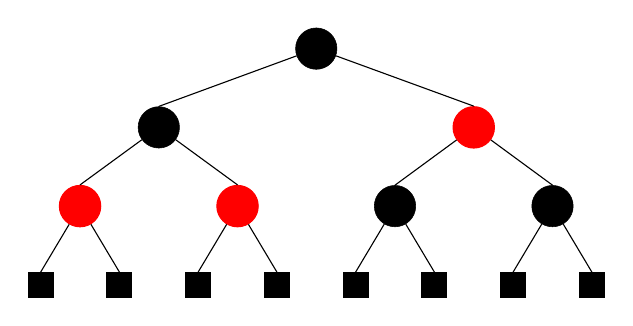
\begin{tikzpicture}
            [-,>=stealth',
            level 1/.style={sibling distance = 4cm, level distance = 1cm},
            level 2/.style={sibling distance = 2cm, level distance = 1cm},
            level 3/.style={sibling distance = 1cm, level distance = 1cm},
            level 4/.style={sibling distance = 0.5cm, level distance = 1cm},
            edge from parent path={(\tikzparentnode) -- (\tikzchildnode.north)}]

            \node 
            [black_node] {}
            child { 
                node [black_node] {}
                child { 
                    node [red_node] {}
                    child{ node [nil] {} }
                    child{ node [nil] {} }
                }
                child { 
                    node [red_node] {}
                    child{ node [nil] {} }
                    child{ node [nil] {} }
                }
            }
            child { 
                node [red_node] {} 
                child { 
                    node [black_node] {} 
                    child{ node [nil] {} }
                    child{ node [nil] {} }
                }
                child { 
                    node [black_node] {}
                    child{ node [nil] {} }
                    child{ node [nil] {} }
                }                            
            }
            ; 
        \end{tikzpicture}
    \end{center}
}

% ===== ADD NODE =====
\newcommand{\ns}{nd}
\newcommand{\setns}[1]{\ifthenelse{\insertslidenumber=1}{\renewcommand{\ns}{ndl}}{}}
\newcommand{\setnum}[1]{\ifthenelse{\insertslidenumber=1}{}{#1}}

% ===== INTERNAL RULE =====
\newcommand{\internalrule} {
    \vspace{-1.5em}
    \begin{flushleft}
        \small{\textbf{Valid}}
    \end{flushleft}
    \vspace{-2em}
    \begin{center}
        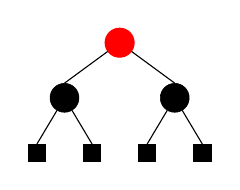
\begin{tikzpicture}
            [-,>=stealth',
            level 1/.style={sibling distance = 2cm, level distance = 1cm},
            level 2/.style={sibling distance = 1cm, level distance = 1cm},
            edge from parent path={(\tikzparentnode) -- (\tikzchildnode.north)}, scale=0.7]

            \node 
            [red_node, scale=0.7] {}
            child { 
                node [black_node, scale=0.7] {}
                child{ node [nil, scale=0.7] {} }
                child{ node [nil, scale=0.7] {} }
            }
            child { 
                node [black_node, scale=0.7] {}
                child{ node [nil, scale=0.7] {} }
                child{ node [nil, scale=0.7] {} }
            }
            ; 
        \end{tikzpicture}
        \hspace{2em}
        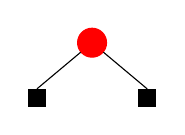
\begin{tikzpicture}
            [-,>=stealth',
            level 1/.style={sibling distance = 2cm, level distance = 1cm},
            level 2/.style={sibling distance = 1cm, level distance = 1cm},
            edge from parent path={(\tikzparentnode) -- (\tikzchildnode.north)}, scale=0.7]

            \node 
            [red_node, scale=0.7] {}
            child{ node [nil, scale=0.7] {} }
            child{ node [nil, scale=0.7] {} }
            ; 
        \end{tikzpicture}
        \vspace{-1em}

    \end{center}
    \hrulefill

    \begin{flushleft}
        \small{\textbf{\textcolor{red}{Invalid}}}
    \end{flushleft}
    \vspace{-2em}
    \begin{center}
        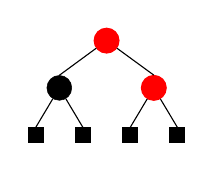
\begin{tikzpicture}
            [-,>=stealth',
            level 1/.style={sibling distance = 2cm, level distance = 1cm},
            level 2/.style={sibling distance = 1cm, level distance = 1cm},
            edge from parent path={(\tikzparentnode) -- (\tikzchildnode.north)}, scale=0.6]

            \node 
            [red_node, scale=0.6] {}
            child { 
                node [black_node, scale=0.6] {}
                child{ node [nil, scale=0.6] {}}
                child{ node [nil, scale=0.6] {}}
            }
            child { 
                node [red_node, scale=0.6] {}
                child{ node [nil, scale=0.6] {}}
                child{ node [nil, scale=0.6] {}}
            }
            ; 
        \end{tikzpicture}
        \hspace{2em}
        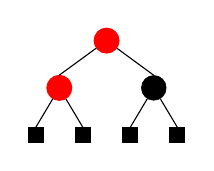
\begin{tikzpicture}
            [-,>=stealth',
            level 1/.style={sibling distance = 2cm, level distance = 1cm},
            level 2/.style={sibling distance = 1cm, level distance = 1cm},
            edge from parent path={(\tikzparentnode) -- (\tikzchildnode.north)}, scale=0.6]

            \node 
            [red_node, scale=0.6] {}
            child { 
                node [red_node, scale=0.6] {}
                child{ node [nil, scale=0.6] {} }
                child{ node [nil, scale=0.6] {} }
            }
            child { 
                node [black_node, scale=0.6] {} 
                child{ node [nil, scale=0.6] {} }
                child{ node [nil, scale=0.6] {} }
            }
            ; 
        \end{tikzpicture}
    \end{center}
}

% ===== EXTERNAL RULE =====
\newcommand{\externalrule} {
    \begin{center}
        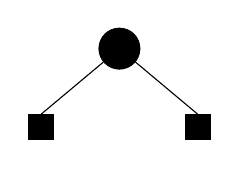
\begin{tikzpicture}
            [-,>=stealth',
            level 1/.style={sibling distance = 2cm, level distance = 1cm},
            level 2/.style={sibling distance = 1cm, level distance = 1cm},
            edge from parent path={(\tikzparentnode) -- (\tikzchildnode.north)}]

            \node 
            [black_node] {}
            child{ node [nil] {} }
            child{ node [nil] {} }
            ; 
        \end{tikzpicture}
    \end{center}
    \begin{center}
        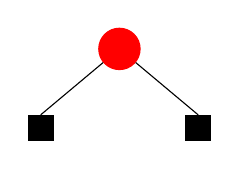
\begin{tikzpicture}
            [-,>=stealth',
            level 1/.style={sibling distance = 2cm, level distance = 1cm},
            level 2/.style={sibling distance = 1cm, level distance = 1cm},
            edge from parent path={(\tikzparentnode) -- (\tikzchildnode.north)}]

            \node 
            [red_node] {}
            child{ node [nil] {} }
            child{ node [nil] {} }
            ; 
        \end{tikzpicture}
    \end{center}
}

% ===== ROOT RULE =====
\newcommand{\rootrule} {
    \begin{center}
        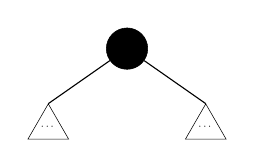
\begin{tikzpicture}
            [-,>=stealth',
            level 1/.style={sibling distance = 2cm, level distance = 1cm},
            level 2/.style={sibling distance = 1cm, level distance = 1cm},
            edge from parent path={(\tikzparentnode) -- (\tikzchildnode.north)}]

            \node 
            [black_node] {}
            child { node [sub] {$\cdots$} }
            child { node [sub] {$\cdots$} }
            ; 
        \end{tikzpicture}
    \end{center}
}

% ===== DEPTH RULE =====
\newcommand{\depthrule} {
    \begin{center}
        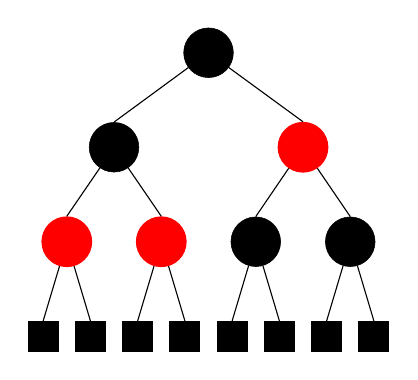
\begin{tikzpicture}
            [-,>=stealth',
            level 1/.style={sibling distance = 2cm, level distance = 1cm},
            level 2/.style={sibling distance = 1cm, level distance = 1cm},
            level 3/.style={sibling distance = 0.5cm, level distance = 1cm},
            edge from parent path={(\tikzparentnode) -- (\tikzchildnode.north)}, scale=1.2]

            \node 
            [black_node, scale=1.2] {}
            child { 
                node [black_node, scale=1.2] {}
                child { 
                    node [red_node, scale=1.2] {}
                    child{ node [nil, scale=1.2] {} }
                    child{ node [nil, scale=1.2] {} }
                }
                child { 
                    node [red_node, scale=1.2] {}
                    child{ node [nil, scale=1.2] {} }
                    child{ node [nil, scale=1.2] {} }
                }
            }
            child { 
                node [red_node, scale=1.2] {} 
                child { 
                    node [black_node, scale=1.2] {} 
                    child{ node [nil, scale=1.2] {} }
                    child{ node [nil, scale=1.2] {} }
                }
                child { 
                    node [black_node, scale=1.2] {}
                    child{ node [nil, scale=1.2] {} }
                    child{ node [nil, scale=1.2] {} }
                }                            
            }
            ; 
        \end{tikzpicture}
    \end{center}
}

% ===== DEPTH EXAMPLE ONE =====
\newcommand{\depthone} {
    \begin{center}
        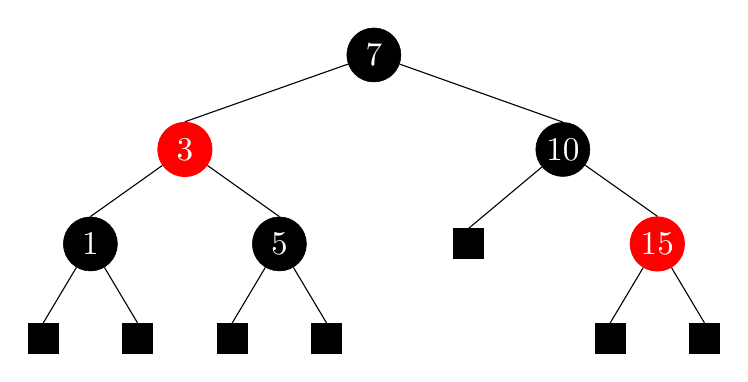
\begin{tikzpicture}
            [-,>=stealth',
            level 1/.style={sibling distance = 4cm, level distance = 1cm},
            level 2/.style={sibling distance = 2cm, level distance = 1cm},
            level 3/.style={sibling distance = 1cm, level distance = 1cm},
            level 4/.style={sibling distance = 0.5cm, level distance = 1cm},
            edge from parent path={(\tikzparentnode) -- (\tikzchildnode.north)}, scale = 1.2]

            \node 
            [black_node, scale = 1.2] {7}
            child { 
                node [red_node, scale = 1.2] {3} 
                child { 
                    node [black_node, scale = 1.2] {1} 
                    child{ node [nil, scale = 1.2] {} }
                    child{ node [nil, scale = 1.2] {} }
                }
                child { 
                    node [black_node, scale = 1.2] {5}
                    child{ node [nil, scale = 1.2] {} }
                    child{ node [nil, scale = 1.2] {} }
                }                            
            }
            child { 
                node [black_node, scale = 1.2] {10}
                child{ node [nil, scale = 1.2] {} }
                child{ node [red_node, scale = 1.2] {15}
                    child{ node [nil, scale = 1.2] {} }
                    child{ node [nil, scale = 1.2] {} }
                }
            }
            ; 
        \end{tikzpicture}
    \end{center}
}

% ===== DEPTH EXAMPLE TWO =====
\newcommand{\depthtwo} {
    \begin{center}
        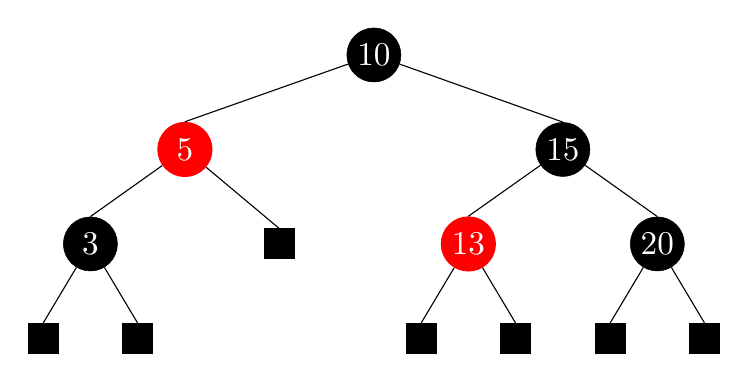
\begin{tikzpicture}
            [-,>=stealth',
            level 1/.style={sibling distance = 4cm, level distance = 1cm},
            level 2/.style={sibling distance = 2cm, level distance = 1cm},
            level 3/.style={sibling distance = 1cm, level distance = 1cm},
            level 4/.style={sibling distance = 0.5cm, level distance = 1cm},
            edge from parent path={(\tikzparentnode) -- (\tikzchildnode.north)}, scale = 1.2]

            \node 
            [black_node, scale = 1.2] {10}
            child { 
                node [red_node, scale = 1.2] {5} 
                child { 
                    node [black_node, scale = 1.2] {3} 
                    child{ node [nil, scale = 1.2] {} }
                    child{ node [nil, scale = 1.2] {} }
                }
                child{ node [nil, scale = 1.2] {} }
            }
            child { 
                node [black_node, scale = 1.2] {15}
                child { 
                    node [red_node, scale = 1.2] {13} 
                    child{ node [nil, scale = 1.2] {} }
                    child{ node [nil, scale = 1.2] {} }
                }
                child { 
                    node [black_node, scale = 1.2] {20}
                    child{ node [nil, scale = 1.2] {} }
                    child{ node [nil, scale = 1.2] {} }
                }
            }
            ;
        \end{tikzpicture}
    \end{center}
}

% ===== DEPTH EXAMPLE THREE =====
\newcommand{\depththree} {
    \begin{center}
        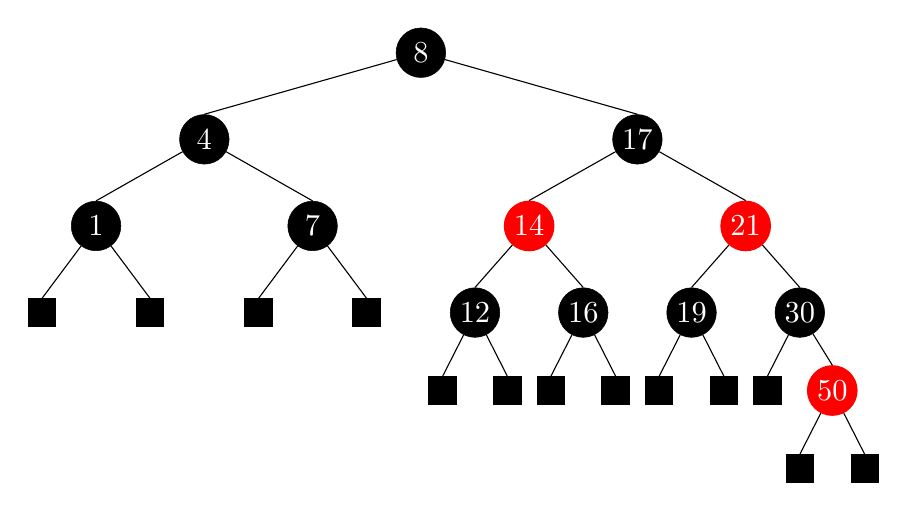
\begin{tikzpicture}
            [-,>=stealth',
            level 1/.style={sibling distance = 5cm, level distance = 1cm},
            level 2/.style={sibling distance = 2.5cm, level distance = 1cm},
            level 3/.style={sibling distance = 1.25cm, level distance = 1cm},
            level 4/.style={sibling distance = 0.75cm, level distance = 0.9cm},
            edge from parent path={(\tikzparentnode) -- (\tikzchildnode.north)}, scale=1.1]

            \node 
            [black_node, scale=1.1] {8}
            child { 
                node [black_node, scale=1.1] {4} 
                child{ node [black_node, scale=1.1] {1} 
                    child{ node [nil, scale=1.1] {} }
                    child{ node [nil, scale=1.1] {} }
                }
                child{ node [black_node, scale=1.1] {7}
                    child{ node [nil, scale=1.1] {} }
                    child{ node [nil, scale=1.1] {} }
                }                            
            }
            child { 
                node [black_node, scale=1.1] {17}
                child { 
                    node [red_node, scale=1.1] {14} 
                    child { 
                        node [black_node, scale=1.1] {12}
                        child{ node [nil, scale=1.1] {} }
                        child{ node [nil, scale=1.1] {} }
                    }                            
                    child { 
                        node [black_node, scale=1.1] {16}
                        child{ node [nil, scale=1.1] {} }
                        child{ node [nil, scale=1.1] {} }
                    }                            
                }
                child { 
                    node [red_node, scale=1.1] {21}
                    child{ 
                        node [black_node, scale=1.1] {19}
                        child{ node [nil, scale=1.1] {} }
                        child{ node [nil, scale=1.1] {} }
                    }
                    child { 
                        node [black_node, scale=1.1] {30}
                        child{ node [nil, scale=1.1] {} }
                        child {
                            node [red_node, scale=1.1] {50}
                            child{ node [nil, scale=1.1] {} }
                            child{ node [nil, scale=1.1] {} }
                        }
                    }                            
                }
            }
            ;
        \end{tikzpicture} 
    \end{center}
}

\newcommand{\doublered} {
    \begin{center}
        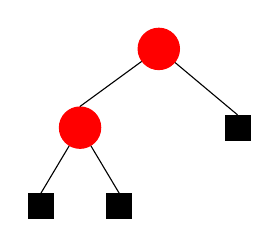
\begin{tikzpicture}
            [-,>=stealth',
            level 1/.style={sibling distance = 2cm, level distance = 1cm},
            level 2/.style={sibling distance = 1cm, level distance = 1cm},
            level 3/.style={sibling distance = 0.5cm, level distance = 1cm},
            edge from parent path={(\tikzparentnode) -- (\tikzchildnode.north)}]

            \node 
            [red_node] {}
            child { 
                node [red_node] {}
                child { node [nil] {}}
                child { node [nil] {}}
            }
            child { node [nil] {}}
            ; 
        \end{tikzpicture}
        \hfil
        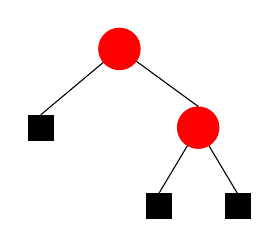
\begin{tikzpicture}
            [-,>=stealth',
            level 1/.style={sibling distance = 2cm, level distance = 1cm},
            level 2/.style={sibling distance = 1cm, level distance = 1cm},
            level 3/.style={sibling distance = 0.5cm, level distance = 1cm},
            edge from parent path={(\tikzparentnode) -- (\tikzchildnode.north)}]

            \node 
            [red_node] {}
            child { node [nil] {}}
            child { 
                node [red_node] {}
                child { node [nil] {}}
                child { node [nil] {}}
            }
            ; 
        \end{tikzpicture}
    \end{center}
}

% ===== RECOLOR BEFORE =====
\newcommand{\recolorbefore} {
    \begin{center}
        \begin{tikzpicture}
            [-,>=stealth',
            level 1/.style={sibling distance = 3cm, level distance = 1cm},
            level 3/.style={sibling distance = 1.5cm, level distance = 1cm},
            level 4/.style={sibling distance = 0.75cm, level distance = 1cm},
            edge from parent path={(\tikzparentnode) -- (\tikzchildnode.north)}]

            \tikzstyle{ndl} = [nil]
            \tikzstyle{nd} = [red_node]

            \node 
            [etc] {$\cdots$}
            child {
                node [black_node] {$10$}
                child { 
                    node [red_node] {$5$} 
                    child { node [nil] {} }
                    child { node [nil] {} }
                }
                child { 
                    node [red_node] {$15$}
                    child { node [nil] {} }
                    child { 
                        node [\ns] {\setnum{$20$}}
                        child [visible on=<2->] { node [nil] {}}
                        child [visible on=<2->] { node [nil] {}}
                    }
                }
            }
            ; 
        \end{tikzpicture}
    \end{center}
}

% ===== RECOLOR AFTER =====
\newcommand{\recolorafter} {
    \begin{center}
        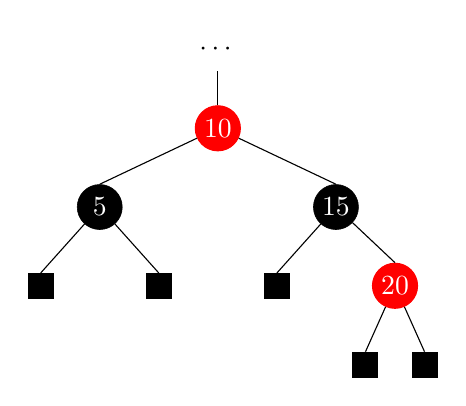
\begin{tikzpicture}
            [-,>=stealth',
            level 1/.style={sibling distance = 3cm, level distance = 1cm},
            level 3/.style={sibling distance = 1.5cm, level distance = 1cm},
            level 4/.style={sibling distance = 0.75cm, level distance = 1cm},
            edge from parent path={(\tikzparentnode) -- (\tikzchildnode.north)}]

            \node 
            [etc] {$\cdots$}
            child {
                node [red_node] {$10$}
                child { 
                    node [black_node] {$5$} 
                    child { node [nil] {} }
                    child { node [nil] {} }
                }
                child { 
                    node [black_node] {$15$}
                    child { node [nil] {} }
                    child { 
                        node [red_node] {$20$}
                        child{ node [nil] {}}
                        child{ node [nil] {}}
                    }
                }
            }
            ; 
        \end{tikzpicture}
    \end{center}
}

% ===== RECOLOR RECURSIVE BEFORE =====
\newcommand{\recolorrecursivebefore} {
    \begin{center}
        \begin{tikzpicture}
            [-,>=stealth',
            level 1/.style={sibling distance = 6cm, level distance = 1cm},
            level 2/.style={sibling distance = 3cm, level distance = 1cm},
            level 3/.style={sibling distance = 1.5cm, level distance = 1cm},
            level 4/.style={sibling distance = 0.75cm, level distance = 1cm},
            level 5/.style={sibling distance = 0.5cm, level distance = 1cm},
            edge from parent path={(\tikzparentnode) -- (\tikzchildnode.north)}]

            \tikzstyle{ndl} = [nil]
            \tikzstyle{nd} = [red_node]

            \node 
            [black_node] {$30$}
            child {
                node [red_node] {$20$}
                child {
                    node [black_node] {$10$}
                    child { 
                        node [red_node] {$5$} 
                        child { node [nil] {} }
                        child { node [nil] {} }
                    }
                    child { 
                        node [red_node] {$15$}
                        child { 
                            node [\ns] {\setnum{$12$}}
                            child [visible on=<2->] { node [nil] {}}
                            child [visible on=<2->] { node [nil] {}}
                        }
                        child { node [nil] {} }
                    }
                }
                child { 
                    node [black_node] {$25$} 
                    child { node [nil] {} }
                    child { node [nil] {} }
                }
            }
            child { 
                node [red_node] {$50$} 
                child { 
                    node [black_node] {$40$} 
                    child { node [nil] {} }
                    child { node [nil] {} }
                }
                child { 
                    node [black_node] {$60$} 
                    child { node [nil] {} }
                    child { node [nil] {} }
                }
            }
            ; 
        \end{tikzpicture}
    \end{center}
}

% ===== RECOLOR RECURSIVE AFTER =====
\newcommand{\recolorrecursiveafter}[4] {
    \begin{center}
        \begin{tikzpicture}
            [-,>=stealth',
            level 1/.style={sibling distance = 6cm, level distance = 1cm},
            level 2/.style={sibling distance = 3cm, level distance = 1cm},
            level 3/.style={sibling distance = 1.5cm, level distance = 1cm},
            level 4/.style={sibling distance = 0.75cm, level distance = 1cm},
            level 5/.style={sibling distance = 0.5cm, level distance = 1cm},
            edge from parent path={(\tikzparentnode) -- (\tikzchildnode.north)}]

            \node 
            [#4] {$30$}
            child {
                node [#3] {$20$}
                child {
                    node [#1] {$10$}
                    child { 
                        node [#2] {$5$} 
                        child { node [nil] {} }
                        child { node [nil] {} }
                    }
                    child { 
                        node [#2] {$15$}
                        child { 
                            node [red_node] {$12$}
                            child{ node [nil] {}}
                            child{ node [nil] {}}
                        }
                        child { node [nil] {} }
                    }
                }
                child { 
                    node [black_node] {$25$} 
                    child { node [nil] {} }
                    child { node [nil] {} }
                }
            }
            child { 
                node [#3] {$50$} 
                child { 
                    node [black_node] {$40$} 
                    child { node [nil] {} }
                    child { node [nil] {} }
                }
                child { 
                    node [black_node] {$60$} 
                    child { node [nil] {} }
                    child { node [nil] {} }
                }
            }
            ; 
        \end{tikzpicture}
    \end{center}
}

% ===== LEFT LEFT SIMPLE BEFORE =====
\newcommand{\llsimplebefore} {
    \begin{center}
        \begin{tikzpicture}
            [-,>=stealth',
            level 1/.style={sibling distance = 3cm, level distance = 1.2cm},
            level 2/.style={sibling distance = 1.5cm, level distance = 1.2cm},
            level 3/.style={sibling distance = 0.75cm, level distance = 1.2cm},
            edge from parent path={(\tikzparentnode) -- (\tikzchildnode.north)}]

            \tikzstyle{ndl} = [nil]
            \tikzstyle{nd} = [red_node]


            \node 
            [black_node] {$3$}
            child { 
                node [red_node] {$2$}
                child{ 
                    node [\ns] {\setnum{$1$}}
                    child [visible on=<2->] { node [nil] {}}
                    child [visible on=<2->] { node [nil] {}}
                }
                child { node [nil] {} }
            }
            child { node [nil] {} }
            ; 
        \end{tikzpicture}
    \end{center}
}

% ===== LEFT LEFT SIMPLE AFTER =====
\newcommand{\llsimpleafter} {
    \begin{center}
        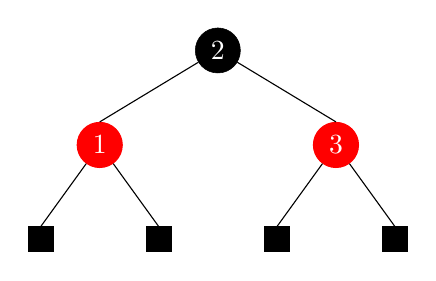
\begin{tikzpicture}
            [-,>=stealth',
            level 1/.style={sibling distance = 3cm, level distance = 1.2cm},
            level 2/.style={sibling distance = 1.5cm, level distance = 1.2cm},
            level 3/.style={sibling distance = 0.75cm, level distance = 1.2cm},
            edge from parent path={(\tikzparentnode) -- (\tikzchildnode.north)}]

            \node 
            [black_node] {$2$}
            child{ 
                node [red_node] {$1$}
                child{ node [nil] {}}
                child{ node [nil] {}}
            }
            child{ 
                node [red_node] {$3$} 
                child { node [nil] {} }
                child { node [nil] {} }
            }
            ; 
        \end{tikzpicture}
    \end{center}
}

% ===== LEFT LEFT GENERAL BEFORE =====
\newcommand{\llbefore} {
    \begin{center}
        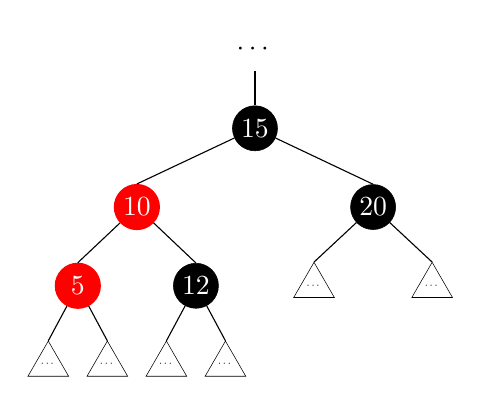
\begin{tikzpicture}
            [-,>=stealth',
            level 1/.style={sibling distance = 3cm, level distance = 1cm},
            level 3/.style={sibling distance = 1.5cm, level distance = 1cm},
            level 4/.style={sibling distance = 0.75cm, level distance = 1cm},
            edge from parent path={(\tikzparentnode) -- (\tikzchildnode.north)}]

            \node 
            [etc] {$\cdots$}
            child {
                node [black_node] {$15$}
                child { 
                    node [red_node] {$10$}
                    child{ 
                        node [red_node] {$5$}
                        child { node [sub] {$\cdots$} }
                        child { node [sub] {$\cdots$} }
                    }
                    child {
                        node [black_node] {$12$} 
                        child { node [sub] {$\cdots$} }
                        child { node [sub] {$\cdots$} }
                    }
                }
                child { 
                    node [black_node] {$20$} 
                    child { node [sub] {$\cdots$} }
                    child { node [sub] {$\cdots$} }
                }
            }
            ; 
        \end{tikzpicture}
    \end{center}
}

% ===== LEFT LEFT GENERAL AFTER =====
\newcommand{\llafter} {
    \begin{center}
        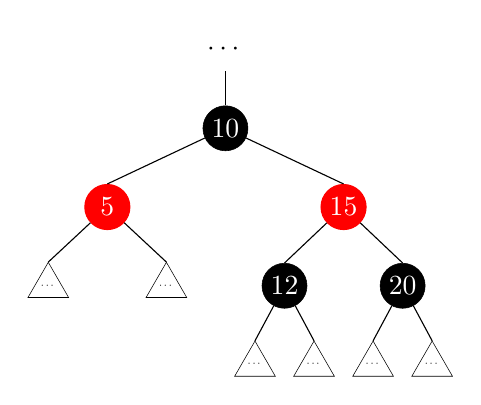
\begin{tikzpicture}
            [-,>=stealth',
            level 1/.style={sibling distance = 3cm, level distance = 1cm},
            level 3/.style={sibling distance = 1.5cm, level distance = 1cm},
            level 4/.style={sibling distance = 0.75cm, level distance = 1cm},
            edge from parent path={(\tikzparentnode) -- (\tikzchildnode.north)}]

            \node 
            [etc] {$\cdots$}
            child {
                node [black_node] {$10$}
                child{ 
                    node [red_node] {$5$}
                    child { node [sub] {$\cdots$} }
                    child { node [sub] {$\cdots$} }
                }
                child{ 
                    node [red_node] {$15$} 
                    child { 
                        node [black_node] {$12$} 
                        child { node [sub] {$\cdots$} }
                        child { node [sub] {$\cdots$} }
                    }
                    child{ 
                        node [black_node] {$20$}
                        child { node [sub] {$\cdots$} }
                        child { node [sub] {$\cdots$} }
                    }
                }
            }
            ; 
        \end{tikzpicture}
    \end{center}
}

% ===== RIGHT RIGHT SIMPLE BEFORE =====
\newcommand{\rrsimplebefore} {
    \begin{center}
        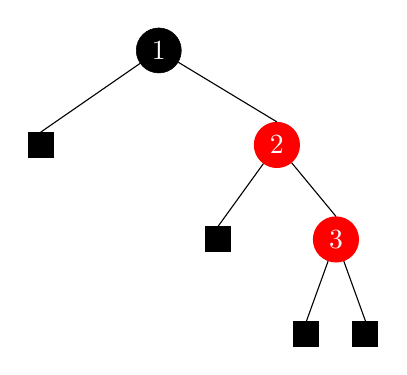
\begin{tikzpicture}
            [-,>=stealth',
            level 1/.style={sibling distance = 3cm, level distance = 1.2cm},
            level 2/.style={sibling distance = 1.5cm, level distance = 1.2cm},
            level 3/.style={sibling distance = 0.75cm, level distance = 1.2cm},
            edge from parent path={(\tikzparentnode) -- (\tikzchildnode.north)}]

            \tikzstyle{ndl} = [nil]
            \tikzstyle{nd} = [red_node]

            \node 
            [black_node] {$1$}
            child { node [nil] {} }
            child { 
                node [red_node] {$2$}
                child { node [nil] {} }
                child{ 
                    node [red_node] {$3$}
                    child { node [nil] {} }
                    child { node [nil] {} }
                }
            }
            ; 
        \end{tikzpicture}
    \end{center}
}

% ===== RIGHT RIGHT SIMPLE AFTER =====
\newcommand{\rrsimpleafter} {
    \begin{center}
        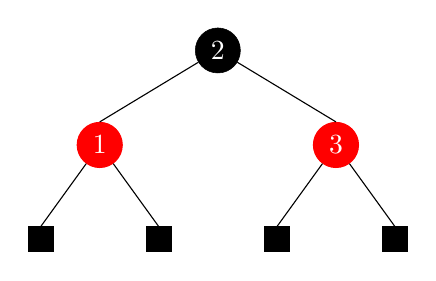
\begin{tikzpicture}
            [-,>=stealth',
            level 1/.style={sibling distance = 3cm, level distance = 1.2cm},
            level 2/.style={sibling distance = 1.5cm, level distance = 1.2cm},
            level 3/.style={sibling distance = 0.75cm, level distance = 1.2cm},
            edge from parent path={(\tikzparentnode) -- (\tikzchildnode.north)}]

            \node 
            [black_node] {$2$}
            child{ 
                node [red_node] {$1$}
                child{ node [nil] {}}
                child{ node [nil] {}}
            }
            child{ 
                node [red_node] {$3$} 
                child { node [nil] {} }
                child { node [nil] {} }
            }
            ; 
        \end{tikzpicture}
    \end{center}
}

% ===== RIGHT RIGHT BEFORE =====
\newcommand{\rrbefore} {
    \begin{center}
        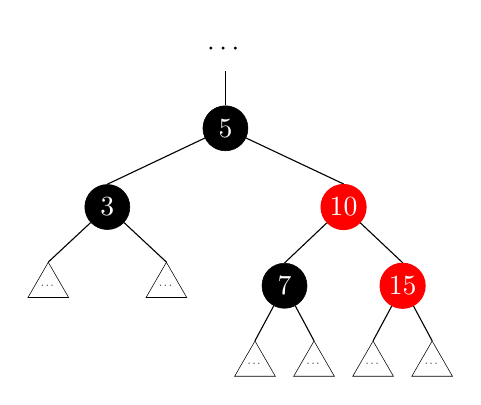
\begin{tikzpicture}
            [-,>=stealth',
            level 1/.style={sibling distance = 3cm, level distance = 1cm},
            level 3/.style={sibling distance = 1.5cm, level distance = 1cm},
            level 4/.style={sibling distance = 0.75cm, level distance = 1cm},
            edge from parent path={(\tikzparentnode) -- (\tikzchildnode.north)}]

            \node 
            [etc] {$\cdots$}
            child {
                node [black_node] {$5$}
                child { 
                    node [black_node] {$3$} 
                    child { node [sub] {$\cdots$} }
                    child { node [sub] {$\cdots$} }
                }
                child { 
                    node [red_node] {$10$}
                    child {
                        node [black_node] {$7$} 
                        child { node [sub] {$\cdots$} }
                        child { node [sub] {$\cdots$} }
                    }
                    child{ 
                        node [red_node] {$15$}
                        child { node [sub] {$\cdots$} }
                        child { node [sub] {$\cdots$} }
                    }
                }
            }
            ; 
        \end{tikzpicture}
    \end{center}
}

% ===== RIGHT RIGHT AFTER =====
\newcommand{\rrafter} {
    \begin{center}
        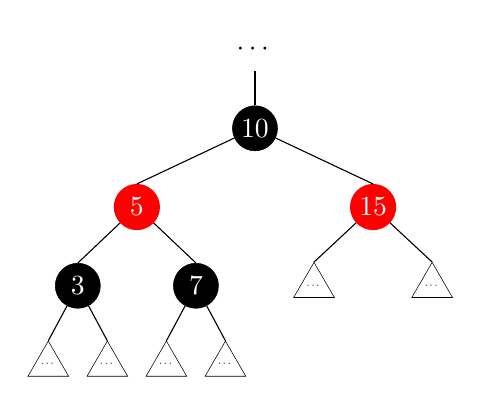
\begin{tikzpicture}
            [-,>=stealth',
            level 1/.style={sibling distance = 3cm, level distance = 1cm},
            level 3/.style={sibling distance = 1.5cm, level distance = 1cm},
            level 4/.style={sibling distance = 0.75cm, level distance = 1cm},
            edge from parent path={(\tikzparentnode) -- (\tikzchildnode.north)}]

            \node 
            [etc] {$\cdots$}
            child {
                node [black_node] {$10$}
                child { 
                    node [red_node] {$5$}
                    child { 
                        node [black_node] {$3$}
                        child { node [sub] {$\cdots$} }
                        child { node [sub] {$\cdots$} }
                    }
                    child { 
                        node [black_node] {$7$} 
                        child { node [sub] {$\cdots$} }
                        child { node [sub] {$\cdots$} }
                    }
                }
                child { 
                    node [red_node] {$15$} 
                    child { node [sub] {$\cdots$} }
                    child { node [sub] {$\cdots$} }
                }
            }
            ; 
        \end{tikzpicture}
    \end{center}
}


% ===== LEFT RIGHT SIMPLE BEFORE =====
\newcommand{\lrsimplebefore} {
    \begin{center}
        \begin{tikzpicture}
            [-,>=stealth',
            level 1/.style={sibling distance = 2cm, level distance = 1cm},
            level 2/.style={sibling distance = 1cm, level distance = 1cm},
            level 3/.style={sibling distance = 0.5cm, level distance = 1cm},
            edge from parent path={(\tikzparentnode) -- (\tikzchildnode.north)}]

            \tikzstyle{ndl} = [nil]
            \tikzstyle{nd} = [red_node]

            \node 
            [black_node] {$3$}
            child{ 
                node [red_node] {$1$}
                child { node [nil] {} }
                child{ 
                    node [\ns] {\setnum{$2$}}
                    child [visible on=<2->] { node [nil] {}}
                    child [visible on=<2->] { node [nil] {}}
                }
            }
            child{ node [nil] {} }
            ; 
        \end{tikzpicture}
    \end{center}
}


% ===== LEFT RIGHT SIMPLE INTERMEDIATE =====
\newcommand{\lrsimpleintermediate} {
    \begin{center}
        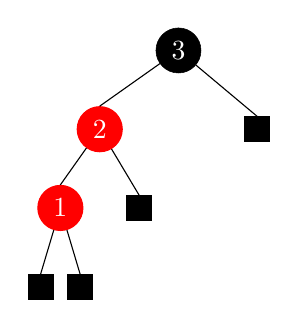
\begin{tikzpicture}
            [-,>=stealth',
            level 1/.style={sibling distance = 2cm, level distance = 1cm},
            level 2/.style={sibling distance = 1cm, level distance = 1cm},
            level 3/.style={sibling distance = 0.5cm, level distance = 1cm},
            edge from parent path={(\tikzparentnode) -- (\tikzchildnode.north)}]

            \node 
            [black_node] {$3$}
            child { 
                node [red_node] {$2$}
                child { 
                    node [red_node] {$1$} 
                    child { node [nil] {} }
                    child { node [nil] {} }
                }
                child { node [nil] {} }
            }
            child { node [nil] {} }
            ; 
        \end{tikzpicture}
    \end{center}
}


% ===== LEFT RIGHT SIMPLE AFTER =====
\newcommand{\lrsimpleafter} {
    \begin{center}
        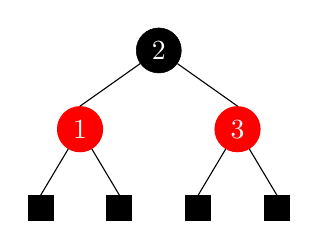
\begin{tikzpicture}
            [-,>=stealth',
            level 1/.style={sibling distance = 2cm, level distance = 1cm},
            level 2/.style={sibling distance = 1cm, level distance = 1cm},
            level 3/.style={sibling distance = 0.5cm, level distance = 1cm},
            edge from parent path={(\tikzparentnode) -- (\tikzchildnode.north)}]

            \node 
            [black_node] {$2$}
            child{ 
                node [red_node] {$1$}
                child { node [nil] {} }
                child{ node [nil] {}}
            }
            child{ 
                node [red_node] {$3$} 
                child{ node [nil] {} }
                child{ node [nil] {} }
            }
            ; 
        \end{tikzpicture}
    \end{center}
}


% ===== LEFT RIGHT BEFORE =====
\newcommand{\lrbefore} {
    \begin{center}
        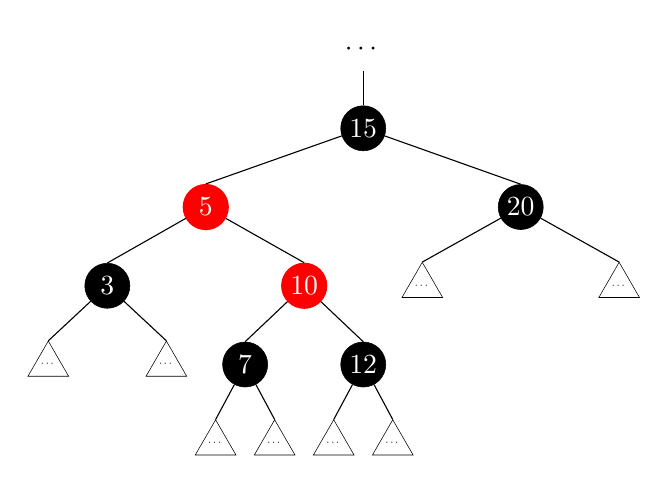
\begin{tikzpicture}
            [-,>=stealth',
            level 1/.style={sibling distance = 4cm, level distance = 1cm},
            level 3/.style={sibling distance = 2.5cm, level distance = 1cm},
            level 4/.style={sibling distance = 1.5cm, level distance = 1cm},
            level 5/.style={sibling distance = 0.75cm, level distance = 1cm},
            edge from parent path={(\tikzparentnode) -- (\tikzchildnode.north)}]

            \node 
            [etc] {$\cdots$}
            child {
                node [black_node] {$15$}
                child { 
                    node [red_node] {$5$}
                    child { 
                        node [black_node] {$3$} 
                        child { node [sub] {$\cdots$} }
                        child { node [sub] {$\cdots$} }
                    }
                    child { 
                        node [red_node] {$10$}
                        child { 
                            node [black_node] {$7$} 
                            child { node [sub] {$\cdots$} }
                            child { node [sub] {$\cdots$} }
                        }
                        child { 
                            node [black_node] {$12$} 
                            child { node [sub] {$\cdots$} }
                            child { node [sub] {$\cdots$} }
                        }
                    }
                }
                child { 
                    node [black_node] {$20$} 
                    child { node [sub] {$\cdots$} }
                    child { node [sub] {$\cdots$} }
                }
            }
            ; 
        \end{tikzpicture}
    \end{center}
}


% ===== LEFT RIGHT INTERMEDIATE =====
\newcommand{\lrintermediate} {
    \begin{center}
        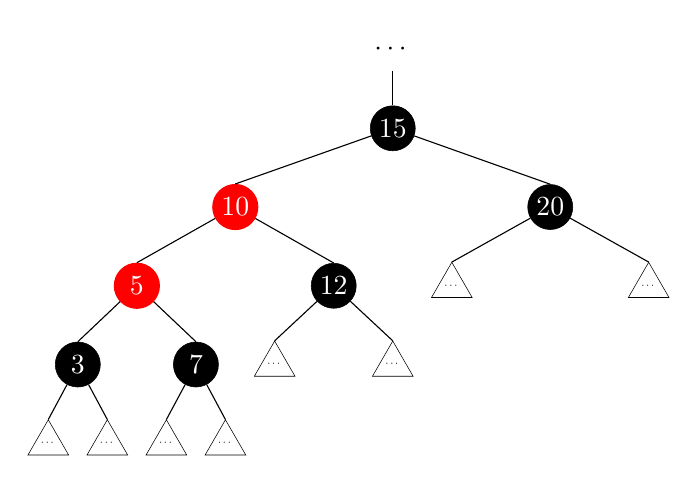
\begin{tikzpicture}
            [-,>=stealth',
            level 1/.style={sibling distance = 4cm, level distance = 1cm},
            level 3/.style={sibling distance = 2.5cm, level distance = 1cm},
            level 4/.style={sibling distance = 1.5cm, level distance = 1cm},
            level 5/.style={sibling distance = 0.75cm, level distance = 1cm},
            edge from parent path={(\tikzparentnode) -- (\tikzchildnode.north)}]

            \node 
            [etc] {$\cdots$}
            child {
                node [black_node] {$15$}
                child { 
                    node [red_node] {$10$}
                    child { 
                        node [red_node] {$5$}
                        child { 
                            node [black_node] {$3$} 
                            child { node [sub] {$\cdots$} }
                            child { node [sub] {$\cdots$} }
                        } 
                        child {
                            node [black_node] {$7$} 
                            child { node [sub] {$\cdots$} }
                            child { node [sub] {$\cdots$} }
                        }
                    }
                    child { 
                        node [black_node] {$12$} 
                        child { node [sub] {$\cdots$} }
                        child { node [sub] {$\cdots$} }
                    }
                }
                child { 
                    node [black_node] {$20$} 
                    child { node [sub] {$\cdots$} }
                    child { node [sub] {$\cdots$} }
                }
            }
            ; 
        \end{tikzpicture}
    \end{center}
}

% ===== LEFT RIGHT AFTER =====
\newcommand{\lrafter} {
    \begin{center}
        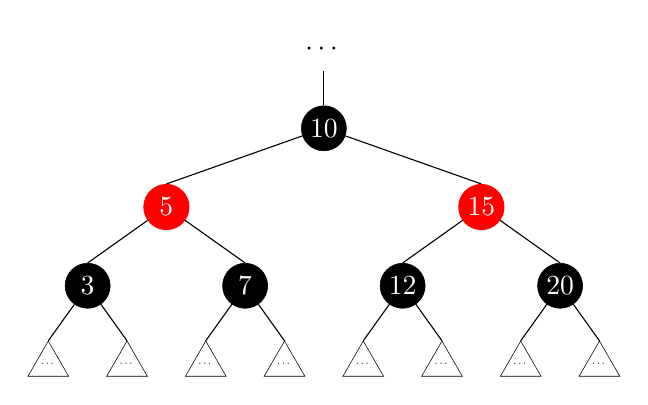
\begin{tikzpicture}
            [-,>=stealth',
            level 1/.style={sibling distance = 4cm, level distance = 1cm},
            level 3/.style={sibling distance = 2cm, level distance = 1cm},
            level 4/.style={sibling distance = 1cm, level distance = 1cm},
            edge from parent path={(\tikzparentnode) -- (\tikzchildnode.north)}]

            \node 
            [etc] {$\cdots$}
            child {
                node [black_node] {$10$}
                child { 
                    node [red_node] {$5$}
                    child { 
                        node [black_node] {$3$} 
                        child { node [sub] {$\cdots$} }
                        child { node [sub] {$\cdots$} }
                    }
                    child {
                        node [black_node] {$7$} 
                        child { node [sub] {$\cdots$} }
                        child { node [sub] {$\cdots$} }
                    }
                }
                child { 
                    node [red_node] {$15$} 
                    child { 
                        node [black_node] {$12$} 
                        child { node [sub] {$\cdots$} }
                        child { node [sub] {$\cdots$} }
                    }
                    child { 
                        node [black_node] {$20$} 
                        child { node [sub] {$\cdots$} }
                        child { node [sub] {$\cdots$} }
                    }
                }
            }
            ; 
        \end{tikzpicture}
    \end{center}
}

% ===== RIGHT LEFT SIMPLE BEFORE =====
\newcommand{\rlsimplebefore} {
    \begin{center}
        \begin{tikzpicture}
            [-,>=stealth',
            level 1/.style={sibling distance = 2cm, level distance = 1cm},
            level 2/.style={sibling distance = 1cm, level distance = 1cm},
            level 3/.style={sibling distance = 0.5cm, level distance = 1cm},
            edge from parent path={(\tikzparentnode) -- (\tikzchildnode.north)}]

            \tikzstyle{ndl} = [nil]
            \tikzstyle{nd} = [red_node]

            \node 
            [black_node] {$1$}
            child{ node [nil] {} }
            child{ 
                node [red_node] {$3$}
                child{ 
                    node [\ns] {\setnum{$2$}}
                    child [visible on=<2->] { node [nil] {}}
                    child [visible on=<2->] { node [nil] {}}
                }
                child { node [nil] {} }
            }
            ; 
        \end{tikzpicture}
    \end{center}
}


% ===== RIGHT LEFT SIMPLE INTERMEDIATE =====
\newcommand{\rlsimpleintermediate} {
    \begin{center}
        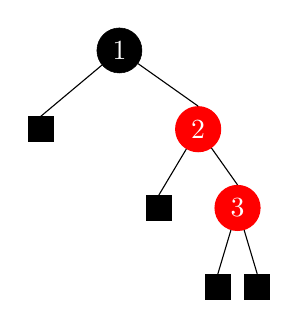
\begin{tikzpicture}
            [-,>=stealth',
            level 1/.style={sibling distance = 2cm, level distance = 1cm},
            level 2/.style={sibling distance = 1cm, level distance = 1cm},
            level 3/.style={sibling distance = 0.5cm, level distance = 1cm},
            edge from parent path={(\tikzparentnode) -- (\tikzchildnode.north)}]

            \node 
            [black_node] {$1$}
            child { node [nil] {} }
            child { 
                node [red_node] {$2$}
                child { node [nil] {} }
                child { 
                    node [red_node] {$3$} 
                    child { node [nil] {} }
                    child { node [nil] {} }
                }
            }
            ; 
        \end{tikzpicture}
    \end{center}
}


% ===== RIGHT LEFT SIMPLE AFTER =====
\newcommand{\rlsimpleafter} {
    \begin{center}
        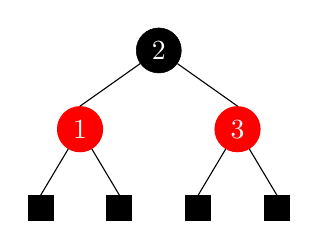
\begin{tikzpicture}
            [-,>=stealth',
            level 1/.style={sibling distance = 2cm, level distance = 1cm},
            level 2/.style={sibling distance = 1cm, level distance = 1cm},
            level 3/.style={sibling distance = 0.5cm, level distance = 1cm},
            edge from parent path={(\tikzparentnode) -- (\tikzchildnode.north)}]

            \node 
            [black_node] {$2$}
            child{ 
                node [red_node] {$1$}
                child { node [nil] {} }
                child{ node [nil] {}}
            }
            child{ 
                node [red_node] {$3$} 
                child{ node [nil] {}}
                child{ node [nil] {}}
            }
            ; 
        \end{tikzpicture}
    \end{center}
}

% ===== RIGHT LEFT BEFORE =====
\newcommand{\rlbefore} {
    \begin{center}
        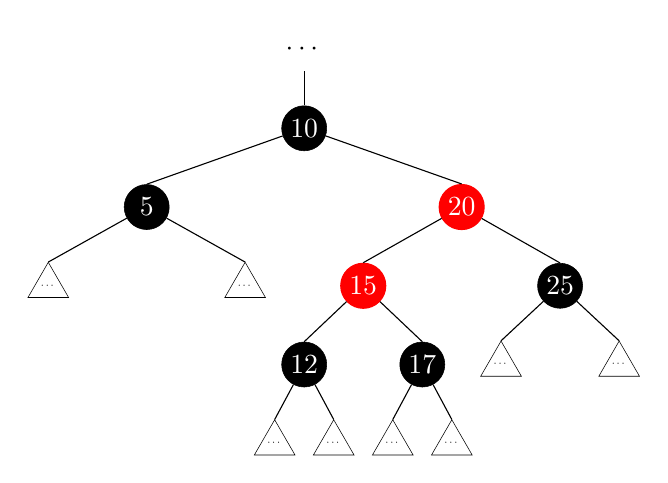
\begin{tikzpicture}
            [-,>=stealth',
            level 1/.style={sibling distance = 4cm, level distance = 1cm},
            level 3/.style={sibling distance = 2.5cm, level distance = 1cm},
            level 4/.style={sibling distance = 1.5cm, level distance = 1cm},
            level 5/.style={sibling distance = 0.75cm, level distance = 1cm},
            edge from parent path={(\tikzparentnode) -- (\tikzchildnode.north)}]

            \node 
            [etc] {$\cdots$}
            child {
                node [black_node] {$10$}
                child { 
                    node [black_node] {$5$} 
                    child { node [sub] {$\cdots$} }
                    child { node [sub] {$\cdots$} }
                }
                child { 
                    node [red_node] {$20$}
                    child { 
                        node [red_node] {$15$}
                        child { 
                            node [black_node] {$12$} 
                            child { node [sub] {$\cdots$} }
                            child { node [sub] {$\cdots$} }
                        }
                        child { 
                            node [black_node] {$17$} 
                            child { node [sub] {$\cdots$} }
                            child { node [sub] {$\cdots$} }
                        }
                    }
                    child { 
                        node [black_node] {$25$} 
                        child { node [sub] {$\cdots$} }
                        child { node [sub] {$\cdots$} }
                    }
                }
            }
            ; 
        \end{tikzpicture}
    \end{center}
}

% ===== LEFT RIGHT INTERMEDIATE =====
\newcommand{\rlintermediate} {
    \begin{center}
        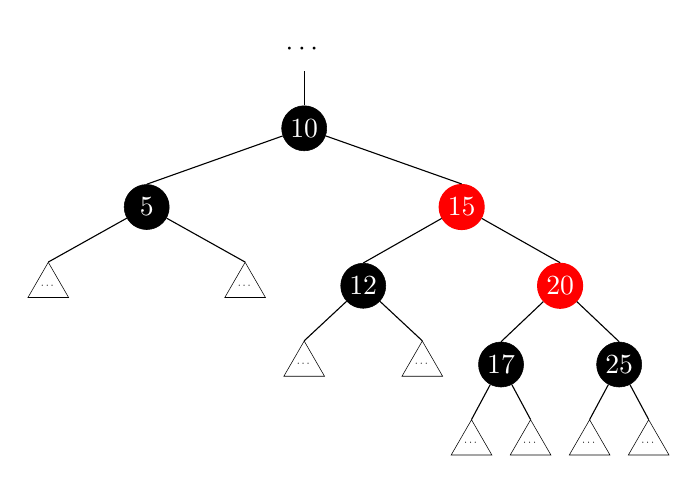
\begin{tikzpicture}
            [-,>=stealth',
            level 1/.style={sibling distance = 4cm, level distance = 1cm},
            level 3/.style={sibling distance = 2.5cm, level distance = 1cm},
            level 4/.style={sibling distance = 1.5cm, level distance = 1cm},
            level 5/.style={sibling distance = 0.75cm, level distance = 1cm},
            edge from parent path={(\tikzparentnode) -- (\tikzchildnode.north)}]

            \node 
            [etc] {$\cdots$}
            child {
                node [black_node] {$10$}
                child { 
                    node [black_node] {$5$} 
                    child { node [sub] {$\cdots$} }
                    child { node [sub] {$\cdots$} }
                }
                child { 
                    node [red_node] {$15$}
                    child { 
                        node [black_node] {$12$} 
                        child { node [sub] {$\cdots$} }
                        child { node [sub] {$\cdots$} }
                    }
                    child { 
                        node [red_node] {$20$}
                        child { 
                            node [black_node] {$17$} 
                            child { node [sub] {$\cdots$} }
                            child { node [sub] {$\cdots$} }
                        }
                        child {
                            node [black_node] {$25$} 
                            child { node [sub] {$\cdots$} }
                            child { node [sub] {$\cdots$} }
                        }
                    }
                }
            }
            ; 
        \end{tikzpicture}
    \end{center}
}

% ===== RIGHT LEFT AFTER =====
\newcommand{\rlafter} {
    \begin{center}
        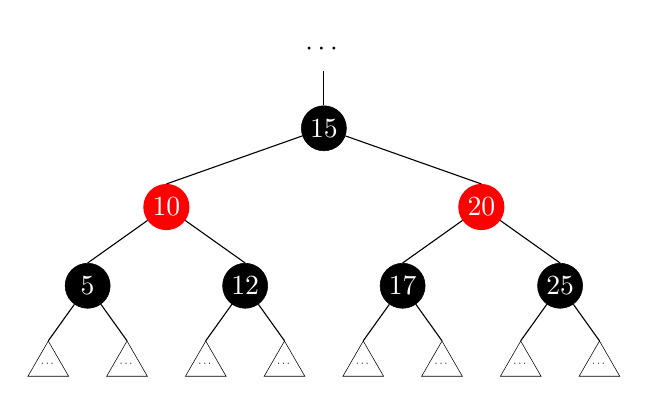
\begin{tikzpicture}
            [-,>=stealth',
            level 1/.style={sibling distance = 4cm, level distance = 1cm},
            level 3/.style={sibling distance = 2cm, level distance = 1cm},
            level 4/.style={sibling distance = 1cm, level distance = 1cm},
            edge from parent path={(\tikzparentnode) -- (\tikzchildnode.north)}]

            \node 
            [etc] {$\cdots$}
            child {
                node [black_node] {$15$}
                child { 
                    node [red_node] {$10$}
                    child { 
                        node [black_node] {$5$} 
                        child { node [sub] {$\cdots$} }
                        child { node [sub] {$\cdots$} }
                    }
                    child {
                        node [black_node] {$12$} 
                        child { node [sub] {$\cdots$} }
                        child { node [sub] {$\cdots$} }
                    }
                }
                child { 
                    node [red_node] {$20$} 
                    child { 
                        node [black_node] {$17$} 
                        child { node [sub] {$\cdots$} }
                        child { node [sub] {$\cdots$} }
                    }
                    child { 
                        node [black_node] {$25$} 
                        child { node [sub] {$\cdots$} }
                        child { node [sub] {$\cdots$} }
                    }
                }
            }
            ; 
        \end{tikzpicture}
    \end{center}
}



\begin{document}
\maketitle

% ===== DEFINITION =====
\begin{frame}[fragile]{Quick Definition}
    \define{
        A \red\textib{-black} tree is a type of \textib{self-balancing} binary search tree that 
        guarantees $\mathcal{O}(\log n)$ performance.
    }
    \exampleone
\end{frame}


% ===== APPLICATIONS =====
\begin{frame}{Applications}
    \textib{\textcolor{red}{Red}-Black} Trees have a variety of applications. Some include:
    \begin{itemize}[label=$\to$]
        % \item Database indexing (2-4 trees\footnote{2-4 (sometimes called 2-3-4) trees are a subset
        %     of B$^+$-trees.} $\simeq$ \red\textib{-black} trees)[e.g. VoltDB]
        \item<2-> Linux CPU scheduler (Completely Fair Scheduler)
        \item<3-> Linux Virtual Memory Areas (VMA)
        \item<4-> STL Data Structures (e.g. C++'s \textmtt{std::map}, Java's \textmtt{HashMap})
        \item<5-> Graph algorithm optimizations (for AI/ML)[e.g. K-mean clustering]
        \item<6-> Priority Queues (e.g. Range Queries)
    \end{itemize}
\end{frame}


% ===== MOTIVATION =====
\begin{frame}{Motivation}
    \textib{Why do we want balanced binary trees?}
    \begin{itemize}[label=$\to$]
        \item<2-> Raw binary search tree performance is highly dependant on input order.
        \item<3-> We want to ensure $\mathcal{O}(\log n)$ performance.
    \end{itemize}
\end{frame}


%===== EXAMPLE ===== 
\begin{frame}[fragile]{Example}
    Suppose we have the input set $\{1, 2, 3, 4, 5, 6, 7\}$ and consider two input orders: \vspace{1em}

    \begin{columns}
        \begin{column}{.5\textwidth}
            \begin{adjustbox}{valign=T, minipage=[t]{\textwidth}}
                \begin{center}
                    $\{1, 2, 3, 4, 5, 6, 7\}$ \vspace{1em}

                    \begin{tikzpicture}[-,>=stealth',level/.style={level distance = 0.8cm},
                        edge from parent path={(\tikzparentnode) -- (\tikzchildnode.north)},
                        grow'=down,every node/.style={node}, scale=0.8]

                        \tikzstyle{ndl} = [nnil, scale=0.5]
                        \tikzstyle{nd} = [scale=0.8]

                        \newcommand{\nsa}{nd}
                        \newcommand{\nsb}{nd}
                        \newcommand{\nsc}{nd}
                        \newcommand{\nsd}{nd}
                        \newcommand{\nse}{nd}
                        \newcommand{\nsf}{nd}
                        \newcommand{\setn}[2]{\ifthenelse{\insertslidenumber=#1}{\renewcommand{#2}{ndl}}{}}
                        \newcommand{\setnumm}[2]{\ifthenelse{\equal{#2}{ndl}}{}{#1}}
                        \setn{1}{\nsa}
                        \setn{2}{\nsb}
                        \setn{3}{\nsc}

                        \node [scale=0.8]
                        {1}
                        child { 
                            node [\nsa] {\setnumm{2}{\nsa}}
                            child [visible on=<2->] { 
                                node [\nsb] {\setnumm{3}{\nsb}} 
                                child [visible on=<3->] { 
                                    node [\nsc] {\setnumm{4}{\nsc}} 
                                    child [visible on = <4->] { 
                                        node [scale=0.8] {5} 
                                        child [visible on=<4->] { 
                                            node [scale = 0.8] {4} 
                                            child [visible on=<4->] { 
                                                node [scale = 0.8] {7} 
                                                child [visible on=<4->] { node [nnil, scale=0.5] {} }
                                                child [visible on=<4->] { node [nnil, scale=0.5] {} }
                                            }
                                            child [visible on=<4->] { node [nnil, scale=0.5] {} }
                                        }
                                        child [visible on=<4->] { node [nnil, scale=0.5] {} }
                                    }
                                    child [visible on=<4->] { node [nnil, scale=0.5] {} }
                                }
                                child [visible on=<3->] { node [nnil, scale=0.5] {} }
                            }
                            child [visible on=<2->] { node [nnil, scale=0.5] {} }
                        }
                        child { node [nnil, scale=0.5] {} }
                        ;
                    \end{tikzpicture}
                \end{center}
            \end{adjustbox}
        \end{column}
        \begin{column}{.5\textwidth}
            \begin{adjustbox}{valign=T, minipage=[t]{\textwidth}}
                \begin{center}
                    $\{1, 7, 2, 6, 3, 5, 4\}$  \vspace{1em}

                    \begin{tikzpicture}[-,>=stealth',level/.style={sibling distance = 5cm/(#1 / 1.2), level distance = 0.8cm},
                        edge from parent path={(\tikzparentnode) -- (\tikzchildnode.north)},
                        grow'=down,every node/.style={node},scale=0.8]
                        \tikzstyle{ndl} = [nnil, scale=0.5]
                        \tikzstyle{nd} = [scale=0.8]

                        \newcommand{\nsa}{nd}
                        \newcommand{\nsb}{nd}
                        \newcommand{\nsc}{nd}
                        \newcommand{\setn}[2]{
                            \pgfmathsetmacro{\result}{#1 + 4}
                            \ifthenelse{\insertslidenumber<\result}{\renewcommand{#2}{ndl}}{}
                        }
                        \newcommand{\setnumm}[2]{\ifthenelse{\equal{#2}{ndl}}{}{#1}}
                        \setn{1}{\nsa}
                        \setn{2}{\nsb}
                        \setn{3}{\nsc}

                        \node [scale=0.8]
                        {1}
                        child { 
                            node [\nsa] {\setnumm{7}{\nsa}} 
                            child [visible on=<5->] { node [nnil, scale=0.5] {} }
                            child [visible on=<5->] { 
                                node [\nsb] {\setnumm{2}{\nsb}} 
                                child [visible on=<6->] { 
                                    node [\nsc] {\setnumm{6}{\nsc}} 
                                    child [visible on=<7>] { node [nnil, scale=0.5] {} }
                                    child [visible on=<7>] { 
                                        node [scale = 0.8] {3} 
                                        child [visible on=<7>] { 
                                            node [scale = 0.8] {5} 
                                            child [visible on=<7>] { node [nnil, scale=0.5] {} }
                                            child [visible on=<7>] { 
                                                node [scale = 0.8] {4} 
                                                child [visible on=<7>] { node [nnil, scale=0.5] {} }
                                                child [visible on=<7>] { node [nnil, scale=0.5] {} }
                                            }
                                        }
                                        child [visible on=<7>] { node [nnil, scale=0.5] {} }
                                    }
                                }
                                child [visible on=<6->] { node [nnil, scale=0.5] {} }
                            }
                        }
                        child { node [nnil, scale=0.5] {} }
                        ;
                    \end{tikzpicture}
                \end{center}
            \end{adjustbox}
        \end{column}
    \end{columns}
\end{frame}


% ===== INTUITION =====
\begin{frame}{Intuition}
    \textib{How do we balance binary trees?} \vspace{1em}

    \onslide<2->{\noindent We can \textit{dynamically} balance the tree!}
    \begin{itemize}[label=$\to$]
        \item<3-> We can add metadata\footnote{Metadata: Additional member variables} to our 
            \textmtt{Node} struct.
        \item<4-> We can define a set of conditions that enforce balance.
    \end{itemize}
\end{frame}


% ===== DEFINITION =====
\begin{frame}[label=def,fragile]{Definition and Properties}
    \define {
        A \red\textib{-black} tree is a type of \textib{self-balancing} binary 
        search tree that guarantees $\mathcal{O}(\log n)$ search, insertion, and deletion operations
        with the following properties:
    }
    \begin{columns}
        \begin{column}{.5\textwidth}
            \begin{adjustbox}{valign=T, minipage=[t]{\textwidth}}
                \begin{enumerate}[label=\textit{(\roman*)}]
                    \item<1> \textit{Color:} Every node is either \red \ or \textib{black}
                    \item<2> \textit{Internal:} A \red \ node does not have a \red \ child
                    \item<3> \textit{External:} All nil nodes are \textib{black}
                    \item<4> \textit{Root:} The root node is always \textib{black}
                    \item<5> \textit{Depth:} Every path from the root to \textit{any} leaf node 
                        passes through the same number of \textib{black} nodes
                \end{enumerate}
            \end{adjustbox}
        \end{column}

        \begin{column}{.5\textwidth}
            \only<1>{\lstinputlisting{struct.tex}}
            \only<2>{\internalrule}
            \only<3>{\externalrule}
            \only<4>{\rootrule}
            \only<5>{\depthrule}
        \end{column}
    \end{columns}
\end{frame}


% ===== DEPTH PROPERTY =====
\begin{frame}[fragile]{Depth Property}
    \vspace{-3em}

    \begin{minipage}[t][0.2\textheight][c]{\linewidth}
        \textit{(v) Depth:} Every path from the root to \textit{any} leaf node passes through the same number 
        of \textib{black} nodes
    \end{minipage}
    \vspace{-3em}

    \begin{minipage}[t][0.6\textheight][c]{\linewidth}
        \setbeamercovered{invisible}
        \only<1> {
            \depthone
            \onslide<1>{\textbf{Valid}}
        }
        \only<3> {\depthtwo}
        \onslide<3> {\textbf{\textcolor{red}{Invalid}}}
        \vspace{1.1em}

        \only<5> {\depththree}
        \onslide<5> {
            \vspace{-2em}
            \textbf{Valid}
        }
    \end{minipage}
\end{frame}

\setbeamercovered{invisible, again covered={\opaqueness<1->{20}}}


% ===== DEFINITION =====
\begin{frame}[fragile]{Definition and Properties}
    \define{
        A \textib{\color{red}{red}}\textib{-black} tree is a type of \textib{self-balancing} binary 
        search tree that guarantees $\mathcal{O}(\log n)$ search, insertion, and deletion operations
        with the following properties:
    }
    \begin{enumerate}[label=\textit{(\roman*)}]
        \item \textit{Color:} Every node is either \red \ or \textib{black}
        \item \textit{Internal:} A \red \ node does not have a \red \ child
        \item \textit{External:} All nil nodes are \textib{black}
        \item \textit{Root}: The root node is always \textib{black}
        \item \textit{Depth:} Every path from the root to \textit{any} leaf node passes through
            the same number of \textib{black} nodes
    \end{enumerate}
\end{frame}


% ===== INSERTION =====
\begin{frame}{Insertion}
    Suppose we have a node $z$ to insert into our \textib{\color{red}{red}}\textib{-black} tree. Then,
    \begin{enumerate}[label=\textit{(\roman*)}]
        \item<2-> Like a BST, insert $z$.
        \item<3-> Color $z$ \red.
        \item<4-> Fix double \red \ violations, if any.
        \item<5-> Recursively fix violations upward.
    \end{enumerate}
\end{frame}


% ===== DOUBLE RED VIOLATION =====
\begin{frame}[fragile]{Double Red Violations}
    Recall \textit{Property (ii): A \red \ node does not have a \red \ child}. \vspace{1em}
    
    When we insert our node $z$ (\red \ by definition), its parent may be \red.
    Below are examples of such cases.
    \doublered
\end{frame}


% ===== FIXING DOUBLE RED VIOLATION =====
\begin{frame}[fragile]{Fixing Double Red Violations}
    \begin{columns}
        \begin{column}{.5\textwidth}
            \textbf{Terminology} \vspace{1em}

            With respect to inserted node $z$,
            \begin{itemize}[label=$\to$]
                \item \textit{Parent} ($p$): $z$'s direct parent
                \item \textit{Uncle} ($u$): $p$'s sibling
                \item \textit{Grandparent} ($g$): $p$'s parent
            \end{itemize}
        \end{column}
        \begin{column}{.5\textwidth}
            \begin{center}
                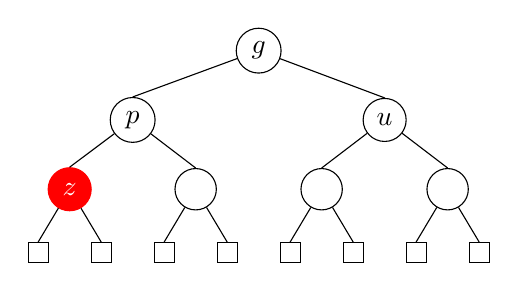
\begin{tikzpicture}
                    [-,>=stealth',
                    level 1/.style={sibling distance = 4cm, level distance = 1.1cm},
                    level 2/.style={sibling distance = 2cm, level distance = 1.1cm},
                    level 3/.style={sibling distance = 1cm, level distance = 1cm},
                    level 4/.style={sibling distance = 0.5cm, level distance = 1.1cm},
                    edge from parent path={(\tikzparentnode) -- (\tikzchildnode.north)},
                    grow' = down,every node/.style = {node}, scale = 0.8]

                    \node {$g$}
                    child { 
                        node {$u$}
                        child {
                            node {}
                            child { node [nnil, scale = 0.8] {} }
                            child { node [nnil, scale = 0.8] {} }
                        }
                        child {
                            node {}
                            child { node [nnil, scale = 0.8] {} }
                            child { node [nnil, scale = 0.8] {} }
                        }
                    }
                    child { 
                        node {$p$}
                        child {
                            node {}
                            child { node [nnil, scale = 0.8] {} }
                            child { node [nnil, scale = 0.8] {} }
                        }
                        child {
                            node [red_node] {$z$}
                            child { node [nnil, scale = 0.8] {} }
                            child { node [nnil, scale = 0.8] {} }
                        }
                    }
                    ;
                \end{tikzpicture}
            \end{center}
        \end{column}
    \end{columns}
    \vspace{2em}

    \onslide<2-> {There are two cases:}
    \begin{enumerate}[label=\textit{(\roman*)}]
        \item<3-> \textib{Recolor:} If both the \textit{parent} and \textit{uncle} are 
            \textib{\color{red}{red}}, perform a \textit{recolor}.
        \item<4-> \textib{Restructure:} If the \textit{parent} is \red \ but the 
            \textit{uncle} is \textib{black}, perform a \textit{tri-node restructure}.
    \end{enumerate}
\end{frame}


% ===== RECOLOR =====
\begin{frame}[fragile]{Recolor}
    \begin{columns}
        \begin{column}{0.45\textwidth}
            \begin{adjustbox}{valign=T, minipage=[t]{\textwidth}}
                \setns{1}
                \recolorbefore
            \end{adjustbox}
        \end{column}
        \onslide<3> {
            \begin{column}{0.1\textwidth}
                \begin{adjustbox}{valign=T, minipage=[t]{\textwidth}}
                    \begin{center}
                        \tikz \draw[-latex] (0,0) -- (1,0);
                    \end{center}
                \end{adjustbox}
            \end{column}
        }
        \onslide<3> {
            \begin{column}{0.45\textwidth}
                \begin{adjustbox}{valign=T, minipage=[t]{\textwidth}}
                    \recolorafter
                \end{adjustbox}
            \end{column}
        }
    \end{columns}
\end{frame}


% ===== RECOLOR RECURSIVE =====
\begin{frame}[fragile]{Recolor (Recursive)}
    \only<1-2>{\setns{1}\recolorrecursivebefore}
    \only<3>{\recolorrecursiveafter{red_node}{black_node}{red_node}{black_node}}
    \only<4>{\recolorrecursiveafter{red_node}{black_node}{black_node}{red_node}}
    \only<5>{\recolorrecursiveafter{red_node}{black_node}{black_node}{black_node}}
\end{frame}

% ===== RESTRUCTURE =====
\begin{frame}{Tri-Node Restructure}
    There are four cases:
    \begin{enumerate}[label=\textit{(\roman*)}]
        \item Left-Left
        \item Right-Right
        \item Left-Right
        \item Right-Left
    \end{enumerate}
\end{frame}


% ===== LEFT LEFT =====
\begin{frame}[fragile]{Case: Left-Left (Simple)}
    \begin{columns}
        \begin{column}{0.45\textwidth}
            \begin{adjustbox}{valign=T, minipage=[t]{\textwidth}}
                \setns{1}
                \llsimplebefore
            \end{adjustbox}
        \end{column}
        \onslide<3> {
            \begin{column}{0.1\textwidth}
                \begin{adjustbox}{valign=T, minipage=[t]{\textwidth}}
                    \begin{center}
                        \tikz \draw[-latex] (0,0) -- (1,0);
                    \end{center}
                \end{adjustbox}
            \end{column}
            \begin{column}{0.45\textwidth}
                \begin{adjustbox}{valign=T, minipage=[t]{\textwidth}}
                    \llsimpleafter
                \end{adjustbox}
            \end{column}
        }
    \end{columns}
\end{frame}


% ===== LEFT LEFT =====
\begin{frame}[fragile]{Case: Left-Left (General)}
    \begin{columns}
        \begin{column}{0.45\textwidth}
            \begin{adjustbox}{valign=T, minipage=[t]{\textwidth}}
                \llbefore
            \end{adjustbox}
        \end{column}
        \onslide<2> {
            \begin{column}{0.1\textwidth}
                \begin{adjustbox}{valign=T, minipage=[t]{\textwidth}}
                    \begin{center}
                        \tikz \draw[-latex] (0,0) -- (1,0);
                    \end{center}
                \end{adjustbox}
            \end{column}
            \begin{column}{0.45\textwidth}
                \begin{adjustbox}{valign=T, minipage=[t]{\textwidth}}
                    \llafter
                \end{adjustbox}
            \end{column}
        }
    \end{columns}
    \vspace{2em}

    Here, 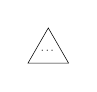
\begin{tikzpicture} \node [sub] {$\cdots$}; \end{tikzpicture} represents a subtree and
    $\cdots$ represents the rest of the tree.
\end{frame}


% ===== RIGHT RIGHT =====
\begin{frame}[fragile]{Case: Right-Right (Simple)}
    \begin{columns}
        \begin{column}{0.45\textwidth}
            \begin{adjustbox}{valign=T, minipage=[t]{\textwidth}}
                \rrsimplebefore
            \end{adjustbox}
        \end{column}
            \begin{column}{0.1\textwidth}
                \begin{adjustbox}{valign=T, minipage=[t]{\textwidth}}
                    \begin{center}
                        \tikz \draw[-latex] (0,0) -- (1,0);
                    \end{center}
                \end{adjustbox}
            \end{column}
            \begin{column}{0.45\textwidth}
                \begin{adjustbox}{valign=T, minipage=[t]{\textwidth}}
                    \rrsimpleafter
                \end{adjustbox}
            \end{column}
    \end{columns}
\end{frame}


% ===== RIGHT RIGHT =====
\begin{frame}[fragile]{Case: Right-Right (General)}
    \begin{columns}
        \begin{column}{0.45\textwidth}
            \begin{adjustbox}{valign=T, minipage=[t]{\textwidth}}
                \rrbefore
            \end{adjustbox}
        \end{column}
            \begin{column}{0.1\textwidth}
                \begin{adjustbox}{valign=T, minipage=[t]{\textwidth}}
                    \begin{center}
                        \tikz \draw[-latex] (0,0) -- (1,0);
                    \end{center}
                \end{adjustbox}
            \end{column}
            \begin{column}{0.45\textwidth}
                \begin{adjustbox}{valign=T, minipage=[t]{\textwidth}}
                    \rrafter
                \end{adjustbox}
            \end{column}
    \end{columns}
    \vspace{2em}

    Here, 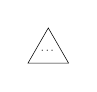
\begin{tikzpicture} \node [sub] {$\cdots$}; \end{tikzpicture} represents a subtree and
    $\cdots$ represents the rest of the tree.
\end{frame}


% ===== LEFT RIGHT =====
\begin{frame}[fragile]{Case: Left-Right (Simple)}
    \begin{columns}
        \begin{column}{0.3\textwidth}
            \begin{adjustbox}{valign=T, minipage=[t]{\textwidth}}
                \setns{1}
                \lrsimplebefore
            \end{adjustbox}
        \end{column}
        \onslide<3-> {
            \begin{column}{0.05\textwidth}
                \begin{adjustbox}{valign=T, minipage=[t]{\textwidth}}
                    \begin{center}
                        \tikz \draw[-latex] (0,0) -- (0.7,0);
                    \end{center}
                \end{adjustbox}
            \end{column}
            \begin{column}{0.3\textwidth}
                \begin{adjustbox}{valign=T, minipage=[t]{\textwidth}}
                    \lrsimpleintermediate
                \end{adjustbox}
            \end{column}
        }
        \onslide<4> {
            \begin{column}{0.05\textwidth}
                \begin{adjustbox}{valign=T, minipage=[t]{\textwidth}}
                    \begin{center}
                        \tikz \draw[-latex] (0,0) -- (0.7,0);
                    \end{center}
                \end{adjustbox}
            \end{column}
            \begin{column}{0.3\textwidth}
                \begin{adjustbox}{valign=T, minipage=[t]{\textwidth}}
                    \lrsimpleafter
                \end{adjustbox}
            \end{column}
        }
    \end{columns}
\end{frame}


% ===== LEFT RIGHT =====
\begin{frame}[fragile]{Case: Left-Right (General)}
    \vspace{-2em}
    \begin{minipage}[t][0.1\textheight][c]{\linewidth}
        \only<1> {\textbf{Step 1}}
        \only<2> {\textbf{Step 2}}
        \only<3> {\textbf{Step 3}}
    \end{minipage}
    \begin{minipage}[t][0.6\textheight][c]{\linewidth}
    \only<1> {\lrbefore}
    \only<2> {\lrintermediate}
    \only<3> {\lrafter}
    \end{minipage}
    \vspace{1em}

    Here, 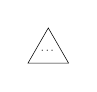
\begin{tikzpicture} \node [sub] {$\cdots$}; \end{tikzpicture} represents a subtree and
    $\cdots$ represents the rest of the tree.
\end{frame}


% ===== RIGHT LEFT =====
\begin{frame}[fragile]{Case: Right-Left (Simple)}
    \begin{columns}
        \begin{column}{0.3\textwidth}
            \begin{adjustbox}{valign=T, minipage=[t]{\textwidth}}
                \rlsimplebefore
            \end{adjustbox}
        \end{column}
        \begin{column}{0.05\textwidth}
            \begin{adjustbox}{valign=T, minipage=[t]{\textwidth}}
                \begin{center}
                    \tikz \draw[-latex] (0,0) -- (0.7,0);
                \end{center}
            \end{adjustbox}
        \end{column}
        \begin{column}{0.3\textwidth}
            \begin{adjustbox}{valign=T, minipage=[t]{\textwidth}}
                \rlsimpleintermediate
            \end{adjustbox}
        \end{column}
        \begin{column}{0.05\textwidth}
            \begin{adjustbox}{valign=T, minipage=[t]{\textwidth}}
                \begin{center}
                    \tikz \draw[-latex] (0,0) -- (0.7,0);
                \end{center}
            \end{adjustbox}
        \end{column}
        \begin{column}{0.3\textwidth}
            \begin{adjustbox}{valign=T, minipage=[t]{\textwidth}}
                \rlsimpleafter
            \end{adjustbox}
        \end{column}
    \end{columns}
\end{frame}


% ===== RIGHT LEFT =====
\begin{frame}[fragile]{Case: Right-Left (General)}
    \begin{columns}
        \begin{column}{0.5\textwidth}
            \begin{adjustbox}{valign=T, minipage=[t]{\textwidth}}
                \rlbefore
            \end{adjustbox}
        \end{column}
        \begin{column}{0.04\textwidth}
            \begin{adjustbox}{valign=T, minipage=[t]{\textwidth}}
                \begin{center}
                    \tikz \draw[-latex] (0,0) -- (0.5,0);
                \end{center}
            \end{adjustbox}
        \end{column}
        \begin{column}{0.46\textwidth}
            \begin{adjustbox}{valign=T, minipage=[t]{\textwidth}}
                \rlafter
            \end{adjustbox}
        \end{column}
    \end{columns}
    \vspace{1em}

    Here, 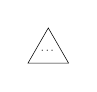
\begin{tikzpicture} \node [sub] {$\cdots$}; \end{tikzpicture} represents a subtree and
    $\cdots$ represents the rest of the tree.
\end{frame}


% ===== TIME AND SPACE COMPLEXITIES =====
\begin{frame}{Time and Space Complexities}
    \begin{itemize}[label=$\to$]
        \item \textib{Insertion}: $\mathcal{O} (\log n)$
        \item \textib{Deletion}: $\mathcal{O} (\log n)$
        \item \textib{Search}: $\mathcal{O} (\log n)$
        \item \textib{Space}: $\mathcal{O} (n)$
\end{itemize}
\end{frame}


% ===== END =====
\begin{frame}{End}
    \begin{center}
        Thank you!
    \end{center}
\end{frame}


% ===== APPENDIX =====
\begin{frame}{Appendix}
    Below are slides that didn't make the cut.
\end{frame}


% ===== COROLLARIES =====
\begin{frame}{Corollaries}
    \proposition{
        If a node $z$ has exactly one child, $c$, then 
        \textnormal{\textbf{(a)}} $c$ is \red,
        \textnormal{\textbf{(b)}} $z$ is \textib{black}, and
        \textnormal{\textbf{(c)}} $c$ has no children.
    }
    \textit{Proof.}
    Suppose we have a valid \red\textib{-black} tree. Consider a node $z$ with exactly one child. 
    Without loss of generality, choose $z$'s left node to be the child and call it $c$.
    \begin{enumerate}[label=\textbf{(\alph*)}]
        \item $z$ passes through no \textib{black} nodes on the right side by assumption. If $c$ were 
            \textib{black}, then $z$ would pass through $1$ \textib{black} node, a contradiction 
            since this violates the \textit{depth property}.
        \item By \textbf{(a)}, $z$'s child is \red \ and by the \textit{internal property}, $z$ is \textib{black}.
        \item Since $z$ passes through no \textib{black} nodes on the right side by assumption,
            $z$ cannot pass through any \textib{black} nodes on the left side by the \textit{the depth
            property}. Then, since $c$ is \red \ by \textbf{(a)}, $c$ has only nil nodes \hfill $\square$
    \end{enumerate}
\end{frame}


\begin{frame}{Height of a Red-Black Tree}
    \thm{
        A \red\textib{-black} tree with $n$ nodes has a height $h$ that is $\mathcal{O} (\log n)$.
    }
    \textit{Proof.}
    Suppose we have a \red\textib{-black} tree with $n$ nodes and height $h$. Let $b$ be the number 
    of \textib{black} nodes on the shortest path from root to any leaf. In the worst case, the 
    longest path alternates between \red \ and \textib{black} nodes and thus has a height of $2b$. 
    Then, $h$ is bounded above by $2b$; that is, $h \leq 2b$. There are $2^b - 1 \leq n$ nodes in 
    this tree. Solving for $b$, we get $b \leq \log(n + 1)$. Substituting $b$, we get 
    $b \leq \log(n + 1) \leq h \leq 2b \leq 2\log(n + 1)$ so $h$ is bounded below by $\log(n + 1)$ 
    and above by $2\log(n + 1)$; that is, $\log(n + 1) \leq h \leq 2\log(n + 1)$. So, $h$ is 
    $\mathcal{O} (\log n)$. \hfill $\square$ 
\end{frame}


% ===== EXAMPLE =====
\begin{frame}[fragile]{Red-Black Tree: Example}
    \begin{center}
        \begin{minipage}{.4\textwidth}
            \begin{center}
                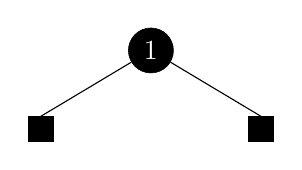
\begin{tikzpicture}[-,>=stealth',level/.style={sibling distance = 2.8cm/#1, level distance = 1cm},
                    edge from parent path={(\tikzparentnode) -- (\tikzchildnode.north)}]
                    \node 
                    [black_node] {$1$}
                    child { node [nil] {} }
                    child { node [nil] {} }
                    ; 
                \end{tikzpicture}
            \end{center}
        \end{minipage}
        \onslide<2>{
            \begin{minipage}{.1\textwidth}
                \begin{center}
                    \tikz \draw[-latex] (0,0) -- (1,0);
                \end{center}
            \end{minipage}
            \begin{minipage}{.4\textwidth}
                \begin{center}
                    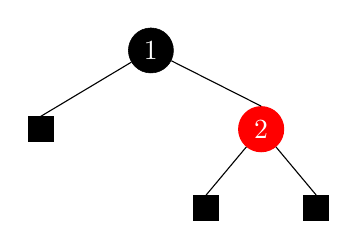
\begin{tikzpicture}[-,>=stealth',level/.style={sibling distance = 2.8cm/#1, level distance = 1cm},
                        edge from parent path={(\tikzparentnode) -- (\tikzchildnode.north)}]
                    \node 
                    [black_node] {$1$}
                    child { node [nil] {} }
                    child { 
                        node [red_node] {$2$} 
                        child { node [nil] {} }
                        child { node [nil] {} }
                    }
                    ; 
                    \end{tikzpicture}
                \end{center}
            \end{minipage}
        }
    \end{center}
\end{frame}

\begin{frame}[fragile]{Red-Black Tree: Example}
    \begin{center}
        \begin{minipage}{.4\textwidth}
            \begin{center}
                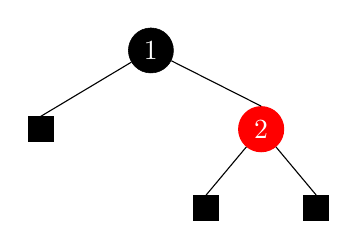
\begin{tikzpicture}[-,>=stealth',level/.style={sibling distance = 2.8cm/#1, level distance = 1cm},
                    edge from parent path={(\tikzparentnode) -- (\tikzchildnode.north)}]
                    \node 
                    [black_node] {$1$}
                    child { node [nil] {} }
                    child { 
                        node [red_node] {$2$} 
                        child { node [nil] {} }
                        child { node [nil] {} }
                    }
                    ; 
                \end{tikzpicture}
            \end{center}
        \end{minipage}
        \onslide<2>{
            \begin{minipage}{.1\textwidth}
                \begin{center}
                    \tikz \draw[-latex] (0,0) -- (1,0);
                \end{center}
            \end{minipage}
            \begin{minipage}{.4\textwidth}
                \begin{center}
                    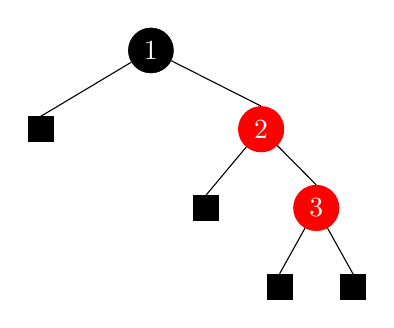
\begin{tikzpicture}[-,>=stealth',level/.style={sibling distance = 2.8cm/#1, level distance = 1cm},
                        edge from parent path={(\tikzparentnode) -- (\tikzchildnode.north)}]
                    \node 
                    [black_node] {$1$}
                    child { node [nil] {} }
                    child { 
                        node [red_node] {$2$} 
                        child { node [nil] {} }
                        child { 
                            node [red_node] {$3$} 
                            child { node [nil] {} }
                            child { node [nil] {} }
                        }
                    }
                    ; 
                    \end{tikzpicture}
                    \newline
                    \hfil
                    \newline
                    \textib{Case: Right-Right}
                \end{center}
            \end{minipage}
        }
    \end{center}
\end{frame}

\begin{frame}[fragile]{Red-Black Tree: Example}
    \begin{center}
        \begin{minipage}{.4\textwidth}
            \begin{center}
                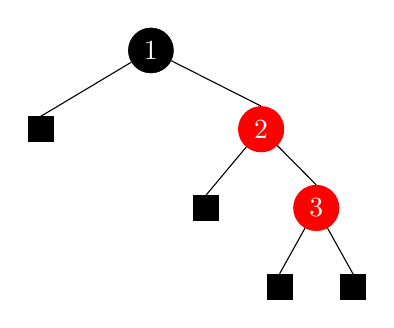
\begin{tikzpicture}[-,>=stealth',level/.style={sibling distance = 2.8cm/#1, level distance = 1cm},
                    edge from parent path={(\tikzparentnode) -- (\tikzchildnode.north)}]
                    \node 
                    [black_node] {$1$}
                    child { node [nil] {} }
                    child { 
                        node [red_node] {$2$} 
                        child { node [nil] {} }
                        child { 
                            node [red_node] {$3$} 
                            child { node [nil] {} }
                            child { node [nil] {} }
                        }
                    }
                    ; 
                \end{tikzpicture}
                \newline
                \hfil
                \newline
                \textib{Case: Right-Right}
            \end{center}
        \end{minipage}
        \onslide<2>{
            \begin{minipage}{.1\textwidth}
                \begin{center}
                    \tikz \draw[-latex] (0,0) -- (1,0);
                \end{center}
            \end{minipage}
            \begin{minipage}{.4\textwidth}
                \begin{center}
                    \begin{tikzpicture}[-,>=stealth',level/.style={sibling distance = 2.8cm/#1, level distance = 1cm},
                        edge from parent path={(\tikzparentnode) -- (\tikzchildnode.north)}]
                        \node 
                        [black_node] {$2$}
                        child { 
                            node [red_node] {$1$} 
                            child { node [nil] {} }
                            child { node [nil] {} }
                        }
                        child { 
                            node [red_node] {$3$} 
                            child { node [nil] {} }
                            child { node [nil] {} }
                        }
                        ; 
                    \end{tikzpicture}
                \end{center}
            \end{minipage}
            }
    \end{center}
\end{frame}

\begin{frame}[fragile]{Red-Black Tree: Example}
    \begin{center}
        \begin{minipage}{.4\textwidth}
            \begin{center}
                \begin{tikzpicture}[-,>=stealth',level/.style={sibling distance = 2.8cm/#1, level distance = 1cm},
                    edge from parent path={(\tikzparentnode) -- (\tikzchildnode.north)}]
                    \node 
                    [black_node] {$2$}
                    child { 
                        node [red_node] {$1$} 
                        child { node [nil] {} }
                        child { node [nil] {} }
                    }
                    child { 
                        node [red_node] {$3$} 
                        child { node [nil] {} }
                        child { node [nil] {} }
                    }
                    ; 
                \end{tikzpicture}
            \end{center}
        \end{minipage}
        \onslide<2>{
            \begin{minipage}{.1\textwidth}
                \begin{center}
                    \tikz \draw[-latex] (0,0) -- (1,0);
                \end{center}
            \end{minipage}
            \begin{minipage}{.4\textwidth}
                \begin{center}
                    \begin{tikzpicture}[-,>=stealth',level/.style={sibling distance = 2.8cm/#1, level distance = 1cm},
                        edge from parent path={(\tikzparentnode) -- (\tikzchildnode.north)}]
                        \node 
                        [black_node] {$2$}
                        child { 
                            node [red_node] {$1$} 
                            child { node [nil] {} }
                            child { node [nil] {} }
                        }
                        child { 
                            node [red_node] {$3$} 
                            child { node [nil] {} }
                            child { 
                                node [red_node] {$4$} 
                                child { node [nil] {} }
                                child { node [nil] {} }
                            }
                        }
                        ; 
                    \end{tikzpicture}
                    \newline
                    \hfil
                    \newline
                    \textib{Case: Recolor}
                \end{center}
            \end{minipage}
            }
    \end{center}
\end{frame}

\begin{frame}[fragile]{Red-Black Tree: Example}
    \begin{center}
        \begin{minipage}{.4\textwidth}
            \begin{center}
                \begin{tikzpicture}[-,>=stealth',level/.style={sibling distance = 2.8cm/#1, level distance = 1cm},
                    edge from parent path={(\tikzparentnode) -- (\tikzchildnode.north)}]
                    \node 
                    [black_node] {$2$}
                    child { 
                        node [red_node] {$1$} 
                        child { node [nil] {} }
                        child { node [nil] {} }
                    }
                    child { 
                        node [red_node] {$3$} 
                        child { node [nil] {} }
                        child { 
                            node [red_node] {$4$} 
                            child { node [nil] {} }
                            child { node [nil] {} }
                        }
                    }
                    ; 
                \end{tikzpicture}
                \newline
                \hfil
                \newline
                \textib{Case: Recolor}
            \end{center}
        \end{minipage}
        \onslide<2>{
            \begin{minipage}{.1\textwidth}
                \begin{center}
                    \tikz \draw[-latex] (0,0) -- (1,0);
                \end{center}
            \end{minipage}
            \begin{minipage}{.4\textwidth}
                \begin{center}
                    \begin{tikzpicture}[-,>=stealth',level/.style={sibling distance = 2.8cm/#1, level distance = 1cm},
                        edge from parent path={(\tikzparentnode) -- (\tikzchildnode.north)}]
                        \node 
                        [black_node] {$2$}
                        child { 
                            node [black_node] {$1$} 
                            child { node [nil] {} }
                            child { node [nil] {} }
                        }
                        child { 
                            node [black_node] {$3$} 
                            child { node [nil] {} }
                            child { 
                                node [red_node] {$4$} 
                                child { node [nil] {} }
                                child { node [nil] {} }
                            }
                        }
                        ; 
                    \end{tikzpicture}
                \end{center}
            \end{minipage}
            }
    \end{center}
\end{frame}

\begin{frame}[fragile]{Red-Black Tree: Example}
    \begin{center}
        \begin{minipage}{.4\textwidth}
            \begin{center}
                \begin{tikzpicture}[-,>=stealth',level/.style={sibling distance = 2.8cm/#1, level distance = 1cm},
                    edge from parent path={(\tikzparentnode) -- (\tikzchildnode.north)}]
                    \node 
                    [black_node] {$2$}
                    child { 
                        node [black_node] {$1$} 
                        child { node [nil] {} }
                        child { node [nil] {} }
                    }
                    child { 
                        node [black_node] {$3$} 
                        child { node [nil] {} }
                        child { 
                            node [red_node] {$4$} 
                            child { node [nil] {} }
                            child { node [nil] {} }
                        }
                    }
                    ; 
                \end{tikzpicture}
            \end{center}
        \end{minipage}
        \onslide<2>{
            \begin{minipage}{.1\textwidth}
                \begin{center}
                    \tikz \draw[-latex] (0,0) -- (1,0);
                \end{center}
            \end{minipage}
            \begin{minipage}{.4\textwidth}
                \begin{center}
                    \begin{tikzpicture}[-,>=stealth',level/.style={sibling distance = 2.8cm/#1, level distance = 1cm},
                        edge from parent path={(\tikzparentnode) -- (\tikzchildnode.north)}]
                        \node 
                        [black_node] {$2$}
                        child { 
                            node [black_node] {$1$} 
                            child { node [nil] {} }
                            child { node [nil] {} }
                        }
                        child { 
                            node [black_node] {$3$} 
                            child { node [nil] {} }
                            child { 
                                node [red_node] {$4$} 
                                child { node [nil] {} }
                                child { 
                                    node [red_node] {$5$} 
                                    child { node [nil] {} }
                                    child { node [nil] {} }
                                }
                            }
                        }
                        ; 
                    \end{tikzpicture}
                    \newline
                    \hfil
                    \newline
                    \textib{Case: Right-Right}
                \end{center}
            \end{minipage}
            }
    \end{center}
\end{frame}

\begin{frame}[fragile]{Red-Black Tree: Example}
    \begin{center}
        \begin{minipage}{.4\textwidth}
            \begin{center}
                \begin{tikzpicture}[-,>=stealth',level/.style={sibling distance = 2.8cm/#1, level distance = 1cm},
                    edge from parent path={(\tikzparentnode) -- (\tikzchildnode.north)}]
                    \node 
                    [black_node] {$2$}
                    child { 
                        node [black_node] {$1$} 
                        child { node [nil] {} }
                        child { node [nil] {} }
                    }
                    child { 
                        node [black_node] {$3$} 
                        child { node [nil] {} }
                        child { 
                            node [red_node] {$4$} 
                            child { node [nil] {} }
                            child { 
                                node [red_node] {$5$} 
                                child { node [nil] {} }
                                child { node [nil] {} }
                            }
                        }
                    }
                    ; 
                \end{tikzpicture}
                \newline
                \hfil
                \newline
                \textib{Case: Right-Right}
            \end{center}
        \end{minipage}
        \onslide<2>{
            \begin{minipage}{.1\textwidth}
                \begin{center}
                    \tikz \draw[-latex] (0,0) -- (1,0);
                \end{center}
            \end{minipage}
            \begin{minipage}{.4\textwidth}
                \begin{center}
                    \begin{tikzpicture}[-,>=stealth',level/.style={sibling distance = 2.8cm/#1, level distance = 1cm},
                        edge from parent path={(\tikzparentnode) -- (\tikzchildnode.north)}]
                        \node 
                        [black_node] {$2$}
                        child { 
                            node [black_node] {$1$} 
                            child { node [nil] {} }
                            child { node [nil] {} }
                        }
                        child { 
                            node [black_node] {$4$} 
                            child { 
                                node [red_node] {$3$} 
                                child { node [nil] {} }
                                child { node [nil] {} }
                            }
                            child { 
                                node [red_node] {$5$} 
                                child { node [nil] {} }
                                child { node [nil] {} }
                            }
                        }
                        ; 
                    \end{tikzpicture}
                \end{center}
            \end{minipage}
            }
    \end{center}
\end{frame}

\begin{frame}[fragile]{Red-Black Tree: Example}
    \begin{center}
        \begin{minipage}{.4\textwidth}
            \begin{center}
                \begin{tikzpicture}[-,>=stealth',level/.style={sibling distance = 2.8cm/#1, level distance = 1cm},
                    edge from parent path={(\tikzparentnode) -- (\tikzchildnode.north)}]
                    \node 
                    [black_node] {$2$}
                    child { 
                        node [black_node] {$1$} 
                        child { node [nil] {} }
                        child { node [nil] {} }
                    }
                    child { 
                        node [black_node] {$4$} 
                        child { 
                            node [red_node] {$3$} 
                            child { node [nil] {} }
                            child { node [nil] {} }
                        }
                        child { 
                            node [red_node] {$5$} 
                            child { node [nil] {} }
                            child { node [nil] {} }
                        }
                    }
                    ; 
                \end{tikzpicture}
            \end{center}
        \end{minipage}
        \onslide<2>{
            \begin{minipage}{.1\textwidth}
                \begin{center}
                    \tikz \draw[-latex] (0,0) -- (1,0);
                \end{center}
            \end{minipage}
            \begin{minipage}{.4\textwidth}
                \begin{center}
                    \begin{tikzpicture}[-,>=stealth',level/.style={sibling distance = 2.8cm/#1, level distance = 1cm},
                        edge from parent path={(\tikzparentnode) -- (\tikzchildnode.north)}]
                        \node 
                        [black_node] {$2$}
                        child { 
                            node [black_node] {$1$} 
                            child { node [nil] {} }
                            child { node [nil] {} }
                        }
                        child { 
                            node [black_node] {$4$} 
                            child { 
                                node [red_node] {$3$} 
                                child { node [nil] {} }
                                child { node [nil] {} }
                            }
                            child { 
                                node [red_node] {$5$} 
                                child { node [nil] {} }
                                child { 
                                    node [red_node] {$6$} 
                                    child { node [nil] {} }
                                    child { node [nil] {} }
                                }
                            }
                        }
                        ; 
                    \end{tikzpicture}
                    \newline
                    \hfil
                    \newline
                    \textib{Case: Recolor}
                \end{center}
            \end{minipage}
            }
    \end{center}
\end{frame}

\begin{frame}[fragile]{Red-Black Tree: Example}
    \begin{center}
        \begin{minipage}{.4\textwidth}
            \begin{center}
                \begin{tikzpicture}[-,>=stealth',level/.style={sibling distance = 2.8cm/#1, level distance = 1cm},
                    edge from parent path={(\tikzparentnode) -- (\tikzchildnode.north)}]
                    \node 
                    [black_node] {$2$}
                    child { 
                        node [black_node] {$1$} 
                        child { node [nil] {} }
                        child { node [nil] {} }
                    }
                    child { 
                        node [black_node] {$4$} 
                        child { 
                            node [red_node] {$3$} 
                            child { node [nil] {} }
                            child { node [nil] {} }
                        }
                        child { 
                            node [red_node] {$5$} 
                            child { node [nil] {} }
                            child { 
                                node [red_node] {$6$} 
                                child { node [nil] {} }
                                child { node [nil] {} }
                            }
                        }
                    }
                    ; 
                \end{tikzpicture}
                \newline
                \hfil
                \newline
                \textib{Case: Recolor}
            \end{center}
        \end{minipage}
        \onslide<2>{
            \begin{minipage}{.1\textwidth}
                \begin{center}
                    \tikz \draw[-latex] (0,0) -- (1,0);
                \end{center}
            \end{minipage}
            \begin{minipage}{.4\textwidth}
                \begin{center}
                    \begin{tikzpicture}[-,>=stealth',level/.style={sibling distance = 2.8cm/#1, level distance = 1cm},
                        edge from parent path={(\tikzparentnode) -- (\tikzchildnode.north)}]
                        \node 
                        [black_node] {$2$}
                        child { 
                            node [black_node] {$1$} 
                            child { node [nil] {} }
                            child { node [nil] {} }
                        }
                        child { 
                            node [red_node] {$4$} 
                            child { 
                                node [black_node] {$3$} 
                                child { node [nil] {} }
                                child { node [nil] {} }
                            }
                            child { 
                                node [black_node] {$5$} 
                                child { node [nil] {} }
                                child { 
                                    node [red_node] {$6$} 
                                    child { node [nil] {} }
                                    child { node [nil] {} }
                                }
                            }
                        }
                        ; 
                    \end{tikzpicture}
                \end{center}
            \end{minipage}
            }
    \end{center}
\end{frame}

\begin{frame}[fragile]{Red-Black Tree: Example}
    \begin{center}
        \begin{minipage}{.4\textwidth}
            \begin{center}
                \begin{tikzpicture}[-,>=stealth',level/.style={sibling distance = 2.8cm/#1, level distance = 1cm},
                    edge from parent path={(\tikzparentnode) -- (\tikzchildnode.north)}]
                    \node 
                    [black_node] {$2$}
                    child { 
                        node [black_node] {$1$} 
                        child { node [nil] {} }
                        child { node [nil] {} }
                    }
                    child { 
                        node [red_node] {$4$} 
                        child { 
                            node [black_node] {$3$} 
                            child { node [nil] {} }
                            child { node [nil] {} }
                        }
                        child { 
                            node [black_node] {$5$} 
                            child { node [nil] {} }
                            child { 
                                node [red_node] {$6$} 
                                child { node [nil] {} }
                                child { node [nil] {} }
                            }
                        }
                    }
                    ; 
                \end{tikzpicture}
            \end{center}
        \end{minipage}
        \onslide<2>{
            \begin{minipage}{.1\textwidth}
                \begin{center}
                    \tikz \draw[-latex] (0,0) -- (1,0);
                \end{center}
            \end{minipage}
            \begin{minipage}{.4\textwidth}
                \begin{center}
                    \begin{tikzpicture}[-,>=stealth',level/.style={sibling distance = 2.8cm/#1, level distance = 1cm},
                        edge from parent path={(\tikzparentnode) -- (\tikzchildnode.north)}, scale=0.8]
                        \node 
                        [black_node, scale=0.8] {$2$}
                        child { 
                            node [black_node, scale=0.8] {$1$} 
                            child { node [nil, scale=0.8] {} }
                            child { node [nil, scale=0.8] {} }
                        }
                        child { 
                            node [red_node, scale=0.8] {$4$} 
                            child { 
                                node [black_node, scale=0.8] {$3$} 
                                child { node [nil, scale=0.8] {} }
                                child { node [nil, scale=0.8] {} }
                            }
                            child { 
                                node [black_node, scale=0.8] {$5$} 
                                child { node [nil, scale=0.8] {} }
                                child { 
                                    node [red_node, scale=0.8] {$6$} 
                                    child { node [nil, scale=0.8] {} }
                                    child { 
                                        node [red_node, scale=0.8] {$7$} 
                                        child { node [nil, scale=0.8] {} }
                                        child { node [nil, scale=0.8] {} }
                                    }
                                }
                            }
                        }
                        ; 
                    \end{tikzpicture}
                    \newline
                    \hfil
                    \newline
                    \textib{Case: Right-Right}
                \end{center}
            \end{minipage}
            }
    \end{center}
\end{frame}

\begin{frame}[fragile]{Red-Black Tree: Example}
    \begin{center}
        \begin{minipage}{.35\textwidth}
            \begin{center}
                \begin{tikzpicture}[-,>=stealth',level/.style={sibling distance = 2.8cm/#1, level distance = 1cm},
                    edge from parent path={(\tikzparentnode) -- (\tikzchildnode.north)}, scale=0.8]
                    \node 
                    [black_node, scale=0.8] {$2$}
                    child { 
                        node [black_node, scale=0.8] {$1$} 
                        child { node [nil, scale=0.8] {} }
                        child { node [nil, scale=0.8] {} }
                    }
                    child { 
                        node [red_node, scale=0.8] {$4$} 
                        child { 
                            node [black_node, scale=0.8] {$3$} 
                            child { node [nil, scale=0.8] {} }
                            child { node [nil, scale=0.8] {} }
                        }
                        child { 
                            node [black_node, scale=0.8] {$5$} 
                            child { node [nil, scale=0.8] {} }
                            child { 
                                node [red_node, scale=0.8] {$6$} 
                                child { node [nil, scale=0.8] {} }
                                child { 
                                    node [red_node, scale=0.8] {$7$} 
                                    child { node [nil, scale=0.8] {} }
                                    child { node [nil, scale=0.8] {} }
                                }
                            }
                        }
                    }
                    ; 
                \end{tikzpicture}
            \end{center}
        \end{minipage}
        \onslide<2>{
            \begin{minipage}{.08\textwidth}
                \begin{center}
                    \tikz \draw[-latex] (0,0) -- (1,0);
                \end{center}
            \end{minipage}
            \begin{minipage}{.45\textwidth}
                \begin{center}
                    \begin{tikzpicture}[-,>=stealth',level/.style={sibling distance = 4cm/#1, level distance = 1cm},
                        edge from parent path={(\tikzparentnode) -- (\tikzchildnode.north)}, scale=0.8]
                        \node 
                        [black_node, scale=0.8] {$2$}
                        child { 
                            node [black_node, scale=0.8] {$1$} 
                            child { node [nil, scale=0.8] {} }
                            child { node [nil, scale=0.8] {} }
                        }
                        child { 
                            node [red_node, scale=0.8] {$4$} 
                            child { 
                                node [black_node, scale=0.8] {$3$} 
                                child { node [nil, scale=0.8] {} }
                                child { node [nil, scale=0.8] {} }
                            }
                            child { 
                                node [black_node, scale=0.8] {$6$} 
                                child { 
                                    node [red_node, scale=0.8] {$5$} 
                                    child { node [nil, scale=0.6] {} }
                                    child { node [nil, scale=0.6] {} }
                                }
                                child { 
                                    node [red_node, scale=0.8] {$7$} 
                                    child { node [nil, scale=0.6] {} }
                                    child { node [nil, scale=0.6] {} }
                                }
                            }
                        }
                        ; 
                    \end{tikzpicture}
                \end{center}
            \end{minipage}
            }
    \end{center}
\end{frame}
\end{document}





% \begin{frame}{Deletion}
%     Suppose we have a node $z$ to delete from our red-black tree.
%     \newline
%     \begin{enumerate}[label=\textit{(\roman*)}]
%         \item If $z$ is a \red leaf node, simply remove $z$.
%         \item If $z$ only has a left child $s$, swap \textit{values} and remove $s$.
%         \item If $z$ has a right child, swap its \textit{value} with its in-order successor $s$ and 
%             remove $s$. 
%     \end{enumerate}
%     \hfil
%     \newline
%     If there is a double \textib{black} in \textit{(ii)} or \textit{(iii)}, perform a 
%     \textit{fixup} at $y$'s original position.
% \end{frame}

% \begin{frame}{Deletion Fixup}
%     There are three cases:
%     \begin{enumerate}[label=\textit{(\roman*)}]
%         \item $y$ has a \red child. Then, we perform a \textib{restructure}.
%         \item $y$'s sibling $w$ is \textib{black}. Then, we perform a \textib{recolor}.
%         \item $y$'s sibling $w$ is \red. Then, we perform an \textib{adjustment} followed by 
%             either case \textit{(ii)} or \textit{(iii)}.
%     \end{enumerate}
% \end{frame}

% \begin{frame}[fragile]{Restructure}
%     \begin{center}
%         \begin{minipage}{.4\textwidth}
%             \begin{center}
%                 \begin{tikzpicture}[-,>=stealth',level/.style={sibling distance = 2.8cm/#1, level distance = 1cm},
%                     edge from parent path={(\tikzparentnode) -- (\tikzchildnode.north)}]
%                     \node 
%                     [black_node] {$x$}
%                     child { 
%                         node [black_node] {$z$} 
%                         child { node [nil] {} }
%                         child { node [nil] {} }
%                     }
%                     child { 
%                         node [black_node] {$y$} 
%                         child { node [nil] {} }
%                         child { 
%                             node [red_node] {$c$} 
%                             child { node [nil] {} }
%                             child { node [nil] {} }
%                         }
%                     }
%                     ; 
%                 \end{tikzpicture}
%             \end{center}
%         \end{minipage}
%         \onslide<2>{
%             \begin{minipage}{.1\textwidth}
%                 \begin{center}
%                     \tikz \draw[-latex] (0,0) -- (1,0);
%                 \end{center}
%             \end{minipage}
%             \begin{minipage}{.4\textwidth}
%                 \begin{center}
%                     \begin{tikzpicture}[-,>=stealth',level/.style={sibling distance = 2.8cm/#1, level distance = 1cm},
%                         edge from parent path={(\tikzparentnode) -- (\tikzchildnode.north)}]
%                         \node 
%                         [black_node] {$y$}
%                         child { 
%                             node [black_node] {$x$} 
%                             child { node [nil] {} }
%                             child { node [nil] {} }
%                         }
%                         child { 
%                             node [black_node] {$c$} 
%                             child { node [nil] {} }
%                             child { node [nil] {} }
%                         }
%                         ; 
%                     \end{tikzpicture}
%                 \end{center}
%             \end{minipage}
%         }
%     \end{center}
%     where
%     \begin{enumerate}[label=,leftmargin=*]
%         \item $z$ is the node to delete
%         \item $y$ is $z$'s sibling 
%         \item $x$ is $y$'s parent
%         \item $c$ is $y$'s child
%     \end{enumerate}
% \end{frame}

% \begin{frame}[fragile]{Restructure}
%     \begin{center}
%         \begin{minipage}{.4\textwidth}
%             \begin{center}
%                 \begin{tikzpicture}[-,>=stealth',level/.style={sibling distance = 2.8cm/#1, level distance = 1cm},
%                     edge from parent path={(\tikzparentnode) -- (\tikzchildnode.north)}]
%                     \node 
%                     [black_node] {$x$}
%                     child { 
%                         node [black_node] {$z$} 
%                         child { node [nil] {} }
%                         child { node [nil] {} }
%                     }
%                     child { 
%                         node [black_node] {$y$} 
%                         child { 
%                             node [red_node] {$c$} 
%                             child { node [nil] {} }
%                             child { node [nil] {} }
%                         }
%                         child { node [nil] {} }
%                     }
%                     ; 
%                 \end{tikzpicture}
%             \end{center}
%         \end{minipage}
%         \onslide<2>{
%             \begin{minipage}{.1\textwidth}
%                 \begin{center}
%                     \tikz \draw[-latex] (0,0) -- (1,0);
%                 \end{center}
%             \end{minipage}
%             \begin{minipage}{.4\textwidth}
%                 \begin{center}
%                     \begin{tikzpicture}[-,>=stealth',level/.style={sibling distance = 2.8cm/#1, level distance = 1cm},
%                         edge from parent path={(\tikzparentnode) -- (\tikzchildnode.north)}]
%                         \node 
%                         [black_node] {$c$}
%                         child { 
%                             node [black_node] {$x$} 
%                             child { node [nil] {} }
%                             child { node [nil] {} }
%                         }
%                         child { 
%                             node [black_node] {$y$} 
%                             child { node [nil] {} }
%                             child { node [nil] {} }
%                         }
%                         ; 
%                     \end{tikzpicture}
%                 \end{center}
%             \end{minipage}
%         }
%     \end{center}
%     where
%     \begin{enumerate}[label=,leftmargin=*]
%         \item $z$ is the node to delete
%         \item $y$ is $z$'s sibling 
%         \item $x$ is $y$'s parent
%         \item $c$ is $y$'s child
%     \end{enumerate}
% \end{frame}



% \begin{frame}[fragile]{Recolor}
%     \begin{center}
%         \begin{minipage}{.4\textwidth}
%             \begin{center}
%                 \begin{tikzpicture}[-,>=stealth',level/.style={sibling distance = 2.8cm/#1, level distance = 1cm},
%                     edge from parent path={(\tikzparentnode) -- (\tikzchildnode.north)}]
%                     \node 
%                     [red_node] {$x$}
%                     child { 
%                         node [black_node] {$y$} 
%                         child { node [nil] {} }
%                         child { node [nil] {} }
%                     }
%                     child { 
%                         node [black_node] {$z$} 
%                         child { node [nil] {} }
%                         child { node [nil] {} }
%                     }
%                     ; 
%                 \end{tikzpicture}
%             \end{center}
%         \end{minipage}
%         \onslide<2>{
%             \begin{minipage}{.1\textwidth}
%                 \begin{center}
%                     \tikz \draw[-latex] (0,0) -- (1,0);
%                 \end{center}
%             \end{minipage}
%             \begin{minipage}{.4\textwidth}
%                 \begin{center}
%                     \begin{tikzpicture}[-,>=stealth',level/.style={sibling distance = 2.8cm/#1, level distance = 1cm},
%                         edge from parent path={(\tikzparentnode) -- (\tikzchildnode.north)}]
%                         \node 
%                         [black_node] {$x$}
%                         child { 
%                             node [red_node] {$y$} 
%                             child { node [nil] {} }
%                             child { node [nil] {} }
%                         }
%                         child { node [nil] {} }
%                         ; 
%                     \end{tikzpicture}
%                 \end{center}
%             \end{minipage}
%         }
%     \end{center}
%     where
%     \begin{enumerate}[label=,leftmargin=*]
%         \item $z$ is the node to delete
%         \item $y$ is $z$'s sibling 
%         \item $x$ is $y$'s parent
%         \item $c$ is $y$'s child
%     \end{enumerate}
% \end{frame}

% \begin{frame}[fragile]{Adjustment}
%     \begin{center}
%         \begin{minipage}{.4\textwidth}
%             \begin{center}
%                 \begin{tikzpicture}[-,>=stealth',level/.style={sibling distance = 2.8cm/#1, level distance = 1cm},
%                     edge from parent path={(\tikzparentnode) -- (\tikzchildnode.north)}]
%                     \node 
%                     [black_node] {$x$}
%                     child { 
%                         node [red_node] {$y$} 
%                         child { 
%                             node [black_node] {$c$} 
%                             child { node [nil] {} }
%                             child { node [nil] {} }
%                         }
%                         child { node [bsub] {$T$} }
%                     }
%                     child { 
%                         node [black_node] {$z$} 
%                         child { node [nil] {} }
%                         child { node [nil] {} }
%                     }
%                     ; 
%                 \end{tikzpicture}
%             \end{center}
%         \end{minipage}
%         \onslide<2>{
%             \begin{minipage}{.1\textwidth}
%                 \begin{center}
%                     \tikz \draw[-latex] (0,0) -- (1,0);
%                 \end{center}
%             \end{minipage}
%             \begin{minipage}{.4\textwidth}
%                 \begin{center}
%                     \begin{tikzpicture}[-,>=stealth',level/.style={sibling distance = 2.8cm/#1, level distance = 1cm},
%                         edge from parent path={(\tikzparentnode) -- (\tikzchildnode.north)}]
%                         \node 
%                         [black_node] {$y$}
%                         child { 
%                             node [black_node] {$c$} 
%                             child { node [nil] {} }
%                             child { node [nil] {} }
%                         }
%                         child { 
%                             node [black_node] {$x$} 
%                             child { node [rsub] {$T$} }
%                             child { node [nil] {} }
%                         }
%                         ; 
%                     \end{tikzpicture}
%                 \end{center}
%             \end{minipage}
%         }
%     \end{center}
%     where
%     \begin{enumerate}[label=,leftmargin=*]
%         \item $z$ is the node to delete
%         \item $y$ is $z$'s sibling 
%         \item $x$ is $y$'s parent
%         \item $c$ is $y$'s child
%     \end{enumerate}
% \end{frame}

% \begin{frame}[fragile]{Case: $y$ is a Leaf Node or has Two \textib{Black} Children}
%     \begin{center}
%         \begin{minipage}{.4\textwidth}
%             \begin{center}
%                 \begin{tikzpicture}[-,>=stealth',level/.style={sibling distance = 2.8cm/#1, level distance = 1cm},
%                     edge from parent path={(\tikzparentnode) -- (\tikzchildnode.north)}]
%                     \node 
%                     [black_node] {$x$}
%                     child{ 
%                         node [black_node] {$y$} 
%                         child { node [nil] {} }
%                         child { node [nil] {} }
%                     }
%                     child{ 
%                         node [black_node] {$w$}
%                         child { node [nil] {} }
%                         child { node [nil] {} }
%                     }
%                     ; 
%                 \end{tikzpicture}
%             \end{center}
%         \end{minipage}
%         \onslide<2>{
%             \begin{minipage}{.1\textwidth}
%                 \begin{center}
%                     \tikz \draw[-latex] (0,0) -- (1,0);
%                 \end{center}
%             \end{minipage}
%             \begin{minipage}{.4\textwidth}
%                 \begin{center}
%                     \begin{tikzpicture}[-,>=stealth',level/.style={sibling distance = 2.8cm/#1, level distance = 1cm},
%                         edge from parent path={(\tikzparentnode) -- (\tikzchildnode.north)}]
%                         \node 
%                         [black_node] {$x$}
%                         child { node [nil] {} }
%                         child{ 
%                             node [red_node] {$w$}
%                             child { node [nil] {} }
%                             child { node [nil] {} }
%                         }
%                         ; 
%                     \end{tikzpicture}
%                 \end{center}
%             \end{minipage}
%         }
%     \end{center}
%     where
%     \begin{enumerate}[label=,leftmargin=*]
%         \item $y$ is the node to delete
%         \item $w$ is $y$'s sibling
%         \item $x$ is $y$'s parent
%     \end{enumerate}
% \end{frame}

% \begin{frame}[fragile]{Case: $y$ has a \textib{\color{red}{Red}} Child}
%     \begin{center}
%         \begin{minipage}{.4\textwidth}
%             \begin{center}
%                 \begin{tikzpicture}[-,>=stealth',level/.style={sibling distance = 2.8cm/#1, level distance = 1cm},
%                     edge from parent path={(\tikzparentnode) -- (\tikzchildnode.north)}, scale=0.7]
%                     \node 
%                     [blue_node, scale=0.7] {$x$}
%                     child{ 
%                         node [black_node, scale=0.7] {$y$} 
%                         child { 
%                             node [red_node, scale=0.7] {$z$} 
%                             child { node [nil, scale=0.7] {} }
%                             child { node [nil, scale=0.7] {} }
%                         }
%                         child { node [nil, scale=0.7] {} }
%                     }
%                     child{ 
%                         node [black_node, scale=0.7] {$w$}
%                         child { node [nil, scale=0.7] {} }
%                         child { node [nil, scale=0.7] {} }
%                     }
%                     ; 
%                 \end{tikzpicture}
%                 \begin{tikzpicture}[-,>=stealth',level/.style={sibling distance = 2.8cm/#1, level distance = 1cm},
%                     edge from parent path={(\tikzparentnode) -- (\tikzchildnode.north)}, scale=0.7]
%                     \node 
%                     [blue_node, scale=0.7] {$x$}
%                     child{ 
%                         node [black_node, scale=0.7] {$y$} 
%                         child { node [nil, scale=0.7] {} }
%                         child { 
%                             node [red_node, scale=0.7] {$z$} 
%                             child { node [nil, scale=0.7] {} }
%                             child { node [nil, scale=0.7] {} }
%                         }
%                     }
%                     child{ 
%                         node [black_node, scale=0.7] {$w$}
%                         child { node [nil, scale=0.7] {} }
%                         child { node [nil, scale=0.7] {} }
%                     }
%                     ; 
%                 \end{tikzpicture}
%             \end{center}
%         \end{minipage}
%         \onslide<2>{
%         \begin{minipage}{.1\textwidth}
%             \begin{center}
%                 \tikz \draw[-latex] (0,0) -- (1,0);
%             \end{center}
%         \end{minipage}
%         \begin{minipage}{.4\textwidth}
%             \begin{center}
%                 \begin{tikzpicture}[-,>=stealth',level/.style={sibling distance = 2.8cm/#1, level distance = 1cm},
%                     edge from parent path={(\tikzparentnode) -- (\tikzchildnode.north)}]
%                     \node 
%                     [red_node] {$x$}
%                     child{ 
%                         node [black_node] {$z$} 
%                         child { node [nil] {} }
%                         child { node [nil] {} }
%                     }
%                     child{ 
%                         node [black_node] {$w$}
%                         child { node [nil] {} }
%                         child { node [nil] {} }
%                     }
%                     ; 
%                 \end{tikzpicture}
%             \end{center}
%         \end{minipage}
%     }
%     \end{center}
%     where
%     \begin{enumerate}[label=,leftmargin=*]
%         \item $y$ is the node to delete
%         \item $w$ is $y$'s sibling
%         \item $x$ is $y$'s parent
%         \item $z$ is $y$'s child
%     \end{enumerate}
% \end{frame}

% \begin{frame}[fragile]{Case: $w$ has a \textib{\color{red}{Red}} Child}
%     \begin{center}
%         \begin{minipage}{.4\textwidth}
%             \begin{center}
%                 \begin{tikzpicture}[-,>=stealth',level/.style={sibling distance = 2.8cm/#1, level distance = 1cm},
%                     edge from parent path={(\tikzparentnode) -- (\tikzchildnode.north)}]
%                     \node 
%                     [blue_node] {$x$}
%                     child{ 
%                         node [black_node] {$y$} 
%                         child { node [nil] {} }
%                         child { node [nil] {} }
%                     }
%                     child{ 
%                         node [black_node] {$w$}
%                         child { node [nil] {} }
%                         child { 
%                             node [red_node] {$z$} 
%                             child { node [nil] {} }
%                             child { node [nil] {} }
%                         }
%                     }
%                     ; 
%                 \end{tikzpicture}
%             \end{center}
%         \end{minipage}
%         \onslide<2>{
%             \begin{minipage}{.1\textwidth}
%                 \begin{center}
%                     \tikz \draw[-latex] (0,0) -- (1,0);
%                 \end{center}
%             \end{minipage}
%             \begin{minipage}{.4\textwidth}
%                 \begin{center}
%                     \begin{tikzpicture}[-,>=stealth',level/.style={sibling distance = 2.8cm/#1, level distance = 1cm},
%                         edge from parent path={(\tikzparentnode) -- (\tikzchildnode.north)}]
%                         \node 
%                         [black_node] {$w$}
%                         child{ 
%                             node [black_node] {$x$} 
%                             child { node [nil] {} }
%                             child { node [nil] {} }
%                         }
%                         child{ 
%                             node [black_node] {$z$}
%                             child { node [nil] {} }
%                             child { node [nil] {} }
%                         }
%                         ; 
%                     \end{tikzpicture}
%                 \end{center}
%             \end{minipage}
%         }
%     \end{center}
%     where
%     \begin{enumerate}[label=,leftmargin=*]
%         \item $y$ is the node to delete
%         \item $z$ is $y$'s child
%         \item $w$ is $y$'s sibling
%         \item $x$ is $y$'s parent
%     \end{enumerate}
% \end{frame}

% \begin{frame}[fragile]{Case: $w$ has a \textib{\color{red}{Red}} Child}
%     \begin{center}
%         \begin{minipage}{.4\textwidth}
%             \begin{center}
%                 \begin{tikzpicture}[-,>=stealth',level/.style={sibling distance = 2.8cm/#1, level distance = 1cm},
%                     edge from parent path={(\tikzparentnode) -- (\tikzchildnode.north)}]
%                     \node 
%                     [blue_node] {$x$}
%                     child{ 
%                         node [black_node] {$y$} 
%                         child { node [nil] {} }
%                         child { node [nil] {} }
%                     }
%                     child{ 
%                         node [black_node] {$w$}
%                         child { 
%                             node [red_node] {$z$} 
%                             child { node [nil] {} }
%                             child { node [nil] {} }
%                         }
%                         child { node [nil] {} }
%                     }
%                     ; 
%                 \end{tikzpicture}
%             \end{center}
%         \end{minipage}
%         \begin{minipage}{.1\textwidth}
%             \begin{center}
%                 \tikz \draw[-latex] (0,0) -- (1,0);
%             \end{center}
%         \end{minipage}
%         \begin{minipage}{.4\textwidth}
%             \begin{center}
%                 \begin{tikzpicture}[-,>=stealth',level/.style={sibling distance = 2.8cm/#1, level distance = 1cm},
%                     edge from parent path={(\tikzparentnode) -- (\tikzchildnode.north)}]
%                     \node 
%                     [black_node] {$z$}
%                     child{ 
%                         node [black_node] {$x$} 
%                         child { node [nil] {} }
%                         child { node [nil] {} }
%                     }
%                     child{ 
%                         node [black_node] {$w$}
%                         child { node [nil] {} }
%                         child { node [nil] {} }
%                     }
%                     ; 
%                 \end{tikzpicture}
%             \end{center}
%         \end{minipage}
%     \end{center}
%     where
%     \begin{enumerate}[label=,leftmargin=*]
%         \item $y$ is the node to delete
%         \item $z$ is $y$'s child
%         \item $w$ is $y$'s sibling
%         \item $x$ is $y$'s parent
%     \end{enumerate}
% \end{frame}


% \begin{frame}[fragile]{Case: $w$ is \textib{\color{red}{Red}}}
%     \begin{center}
%         \begin{minipage}{.4\textwidth}
%             \begin{center}
%                 \begin{tikzpicture}[-,>=stealth',level/.style={sibling distance = 2.8cm/#1, level distance = 1cm},
%                     edge from parent path={(\tikzparentnode) -- (\tikzchildnode.north)}]
%                     \node 
%                     [black_node] {$x$}
%                     child{ 
%                         node [black_node] {$y$} 
%                         child { node [nil] {} }
%                         child { node [nil] {} }
%                     }
%                     child{ 
%                         node [red_node] {$w$}
%                         child { node [bsub] {$T$} }
%                         child { 
%                             node [black_node] {$z$} 
%                             child { node [nil] {} }
%                             child { node [nil] {} }
%                         }
%                     }
%                     ; 
%                 \end{tikzpicture}
%             \end{center}
%         \end{minipage}
%         \onslide<2>{
%             \begin{minipage}{.1\textwidth}
%                 \begin{center}
%                     \tikz \draw[-latex] (0,0) -- (1,0);
%                 \end{center}
%             \end{minipage}
%             \begin{minipage}{.4\textwidth}
%                 \begin{center}
%                     \begin{tikzpicture}[-,>=stealth',level/.style={sibling distance = 2.8cm/#1, level distance = 1cm},
%                         edge from parent path={(\tikzparentnode) -- (\tikzchildnode.north)}]
%                         \node 
%                         [black_node] {$w$}
%                         child{ 
%                             node [black_node] {$x$} 
%                             child { node [nil] {} }
%                             child { node [rsub] {$T$} }
%                         }
%                         child{ 
%                             node [black_node] {$z$}
%                             child { node [nil] {} }
%                             child { node [nil] {} }
%                         }
%                         ; 
%                     \end{tikzpicture}
%                 \end{center}
%             \end{minipage}
%         }
%     \end{center}
%     where
%     \begin{enumerate}[label=,leftmargin=*]
%         \item $y$ is the node to delete
%         \item $z$ is $y$'s child
%         \item $w$ is $y$'s sibling
%         \item $x$ is $y$'s parent
%         \item $T$ is $w$'s subtree \end{enumerate}
% \end{frame}

%  \begin{frame}[fragile]{Red-Black Tree Example}
%     \begin{center}
%         \begin{tikzpicture}[-,>=stealth',level/.style={sibling distance = 6cm/#1, level distance = 1.5cm},
%             edge from parent path={(\tikzparentnode) -- (\tikzchildnode.north)}]
%             \node [black_node] {25}
%                 child{ node [red_node] {21} 
%                     child{ node [black_node] {18} 
%                         child{ node [red_node] {2} 
%                             child{ node [nil] {} }
%                             child{ node [nil] {} }
%                         }
%                         child{ node [nil] {} }
%                     }
%                     child{ node [black_node] {24}
%                         child{ node [red_node] {22}
%                             child{ node [nil] {} }
%                             child{ node [nil] {} }
%                         }
%                         child{ node [nil] {} }
%                     }                            
%                 }
%                 child{ node [red_node] {50}
%                     child{ node [black_node] {35} 
%                         child{ node [red_node] {33}
%                             child{ node [nil] {} }
%                             child{ node [nil] {} }
%                         }
%                         child{ node [nil] {} }
%                     }
%                     child{ node [black_node] {52}
%                         child{ node [nil] {} }
%                         child{ node [nil] {} }
%                     }
%                 }
%                 ; 
%         \end{tikzpicture}
%     \end{center}
% \end{frame}
% \begin{frame}[fragile]{Example: Input order \textit{(i)}}
%     \textit{(i)} $\{1, 2, 3, 4, 5, 6, 7\}$ 
%     \begin{center}
%         \begin{tikzpicture}[-,>=stealth',level/.style={level distance = 0.8cm},
%             edge from parent path={(\tikzparentnode) -- (\tikzchildnode.north)},grow'=down,every node/.style={node}]
%             \node 
%             {1}
%             child { 
%                 node {2}
%                 child { 
%                     node {3} 
%                     child { 
%                         node {4} 
%                         child { 
%                             node {5} 
%                             child { 
%                                 node {6} 
%                                 child { 
%                                     node {7} 
%                                     child { node [nnil] {} }
%                                     child { node [nnil] {} }
%                                 }
%                                 child { node [nnil] {} }
%                             }
%                             child { node [nnil] {} }
%                         }
%                         child { node [nnil] {} }
%                     }
%                     child { node [nnil] {} }
%                 }
%                 child { node [nnil] {} }
%             }
%             child { 
%                 node [nnil] {}
%             }
%             ;
%         \end{tikzpicture}
%     \end{center}
% \end{frame}

% \begin{frame}[fragile]{Example: Input order \textit{(ii)}}
%     \textit{(ii)} $\{1, 7, 2, 6, 3, 5, 4\}$ 
%     \begin{center}
%         \begin{tikzpicture}[-,>=stealth',level/.style={sibling distance = 5cm/(#1 / 1.5), level distance = 0.8cm},
%             edge from parent path={(\tikzparentnode) -- (\tikzchildnode.north)},grow'=down,every node/.style={node}]
%             \node 
%             {1}
%             child { 
%                 node {7} 
%                 child { node [nnil] {} }
%                 child { 
%                     node {2} 
%                     child { 
%                         node {6} 
%                         child { node [nnil] {} }
%                         child { 
%                             node {3} 
%                             child { 
%                                 node {5} 
%                                 child { node [nnil] {} }
%                                 child { 
%                                     node {4} 
%                                     child { node [nnil] {} }
%                                     child { node [nnil] {} }
%                                 }
%                             }
%                             child { node [nnil] {} }
%                         }
%                     }
%                     child { node [nnil] {} }
%                 }
%             }
%             child { node [nnil] {} }
%             ;
%         \end{tikzpicture}
%     \end{center}
% \end{frame}

% \begin{frame}[fragile]{Example: Input order \textit{(ii)}}
%     \textit{(ii)} $\{4, 2, 6, 1, 5, 3, 7\}$ 
%     \begin{center}
%         \begin{tikzpicture}[-,>=stealth',level/.style={sibling distance = 5cm/#1, level distance = 1.5cm},
%             edge from parent path={(\tikzparentnode) -- (\tikzchildnode.north)},grow'=down,every node/.style={node}]
%             \node 
%             {4}
%             child { 
%                 node {6} 
%                 child { 
%                     node {7} 
%                     child { node [nnil] {} }
%                     child { node [nnil] {} }
%                 }
%                 child { 
%                     node {5} 
%                     child { node [nnil] {} }
%                     child { node [nnil] {} }
%                 }
%             }
%             child { 
%                 node {2} 
%                 child { 
%                     node {3} 
%                     child { node [nnil] {} }
%                     child { node [nnil] {} }
%                 }
%                 child { 
%                     node {1} 
%                     child { node [nnil] {} }
%                     child { node [nnil] {} }
%                 }
%             }
%             ;
%         \end{tikzpicture}
%     \end{center}
% \end{frame}

% ===== EXAMPLE =====
% \begin{frame}[fragile]{Example: Rotation around $2$}
%     \centering
%     \begin{minipage}{.4\textwidth}
%         \centering
%         \begin{tikzpicture}[-,>=stealth',level/.style={level distance = 0.8cm},
%             edge from parent path={(\tikzparentnode) -- (\tikzchildnode.north)},grow'=down,every node/.style={node}]
%             \node 
%             {1}
%             child { 
%                 node {2}
%                 child { 
%                     node {3} 
%                     child { node [nnil] {} }
%                     child { node [sub] {$\beta$} }
%                 }
%                 child { node [sub] {$\alpha$} }
%             }
%             child { 
%                 node [nnil] {}
%             }
%             ;
%         \end{tikzpicture}
%     \end{minipage}
%     \begin{minipage}{.1\textwidth}
%         \centering
%         \tikz \draw[-latex] (0,0) -- (1,0);
%     \end{minipage}
%     \begin{minipage}{.4\textwidth}
%         \centering
%         \begin{tikzpicture}[-,>=stealth',level/.style={sibling distance = 3cm/#1, level distance = 1cm},
%             edge from parent path={(\tikzparentnode) -- (\tikzchildnode.north)},grow'=down,every node/.style={node}]
%             \node 
%             {2}
%             child { 
%                 node {3}
%                 child { node [nnil] {} }
%                 child { node [sub] {$\beta$} }
%             }
%             child { 
%                 node {1} 
%                 child { node [sub] {$\alpha$} }
%                 child { node [nnil] {} }
%             }
%             ;
%         \end{tikzpicture}
%     \end{minipage}
% \end{frame}
